\documentclass[twoside]{book}

% Packages required by doxygen
\usepackage{fixltx2e}
\usepackage{calc}
\usepackage{doxygen}
\usepackage[export]{adjustbox} % also loads graphicx
\usepackage{graphicx}
\usepackage[utf8]{inputenc}
\usepackage{makeidx}
\usepackage{multicol}
\usepackage{multirow}
\PassOptionsToPackage{warn}{textcomp}
\usepackage{textcomp}
\usepackage[nointegrals]{wasysym}
\usepackage[table]{xcolor}

% Font selection
\usepackage[T1]{fontenc}
\usepackage[scaled=.90]{helvet}
\usepackage{courier}
\usepackage{amssymb}
\usepackage{sectsty}
\renewcommand{\familydefault}{\sfdefault}
\allsectionsfont{%
  \fontseries{bc}\selectfont%
  \color{darkgray}%
}
\renewcommand{\DoxyLabelFont}{%
  \fontseries{bc}\selectfont%
  \color{darkgray}%
}
\newcommand{\+}{\discretionary{\mbox{\scriptsize$\hookleftarrow$}}{}{}}

% Page & text layout
\usepackage{geometry}
\geometry{%
  a4paper,%
  top=2.5cm,%
  bottom=2.5cm,%
  left=2.5cm,%
  right=2.5cm%
}
\tolerance=750
\hfuzz=15pt
\hbadness=750
\setlength{\emergencystretch}{15pt}
\setlength{\parindent}{0cm}
\setlength{\parskip}{3ex plus 2ex minus 2ex}
\makeatletter
\renewcommand{\paragraph}{%
  \@startsection{paragraph}{4}{0ex}{-1.0ex}{1.0ex}{%
    \normalfont\normalsize\bfseries\SS@parafont%
  }%
}
\renewcommand{\subparagraph}{%
  \@startsection{subparagraph}{5}{0ex}{-1.0ex}{1.0ex}{%
    \normalfont\normalsize\bfseries\SS@subparafont%
  }%
}
\makeatother

% Headers & footers
\usepackage{fancyhdr}
\pagestyle{fancyplain}
\fancyhead[LE]{\fancyplain{}{\bfseries\thepage}}
\fancyhead[CE]{\fancyplain{}{}}
\fancyhead[RE]{\fancyplain{}{\bfseries\leftmark}}
\fancyhead[LO]{\fancyplain{}{\bfseries\rightmark}}
\fancyhead[CO]{\fancyplain{}{}}
\fancyhead[RO]{\fancyplain{}{\bfseries\thepage}}
\fancyfoot[LE]{\fancyplain{}{}}
\fancyfoot[CE]{\fancyplain{}{}}
\fancyfoot[RE]{\fancyplain{}{\bfseries\scriptsize Generated by Doxygen }}
\fancyfoot[LO]{\fancyplain{}{\bfseries\scriptsize Generated by Doxygen }}
\fancyfoot[CO]{\fancyplain{}{}}
\fancyfoot[RO]{\fancyplain{}{}}
\renewcommand{\footrulewidth}{0.4pt}
\renewcommand{\chaptermark}[1]{%
  \markboth{#1}{}%
}
\renewcommand{\sectionmark}[1]{%
  \markright{\thesection\ #1}%
}

% Indices & bibliography
\usepackage{natbib}
\usepackage[titles]{tocloft}
\setcounter{tocdepth}{3}
\setcounter{secnumdepth}{5}
\makeindex

% Hyperlinks (required, but should be loaded last)
\usepackage{ifpdf}
\ifpdf
  \usepackage[pdftex,pagebackref=true]{hyperref}
\else
  \usepackage[ps2pdf,pagebackref=true]{hyperref}
\fi
\hypersetup{%
  colorlinks=true,%
  linkcolor=blue,%
  citecolor=blue,%
  unicode%
}

% Custom commands
\newcommand{\clearemptydoublepage}{%
  \newpage{\pagestyle{empty}\cleardoublepage}%
}

\usepackage{caption}
\captionsetup{labelsep=space,justification=centering,font={bf},singlelinecheck=off,skip=4pt,position=top}

%===== C O N T E N T S =====

\begin{document}

% Titlepage & ToC
\hypersetup{pageanchor=false,
             bookmarksnumbered=true,
             pdfencoding=unicode
            }
\pagenumbering{roman}
\begin{titlepage}
\vspace*{7cm}
\begin{center}%
{\Large thenable \\[1ex]\large 0.\+1 }\\
\vspace*{1cm}
{\large Generated by Doxygen 1.8.11}\\
\end{center}
\end{titlepage}
\clearemptydoublepage
\tableofcontents
\clearemptydoublepage
\pagenumbering{arabic}
\hypersetup{pageanchor=true}

%--- Begin generated contents ---
\chapter{thenable}
\label{index}\hypertarget{index}{}\begin{quote}
\char`\"{}\+There is a point where we needed to stop and we have clearly passed it but let’s keep going and see what happens.\char`\"{} \end{quote}


This is a generic implementation of {\ttfamily then} for C++14, allowing you to chain together futures, promises and so forth easily and efficiently.

\#\# Example\+: 
\begin{DoxyCode}
1 \{C++\}
2 #include "thenable.hpp"
3 
4 #include <iostream>
5 #include <chrono>
6 #include <thread>
7 #include <assert.h>
8 
9 using namespace std;
10 using namespace thenable;
11 
12 int main() \{
13     ThenablePromise<int> p, k;
14 
15     cout << "Starting asynchronous tasks on thread: " << this\_thread::get\_id() << endl;
16 
17     p.then( [&k]( int i ) \{
18         assert( i == 10 );
19 
20         cout << "Hello, World! from thread: " << this\_thread::get\_id() << endl;
21 
22         k.set\_value( 421 );
23 
24         return k.get\_future();
25 
26     \} ).then( []( int i ) \{
27         assert( i = 421 );
28 
29         cout << "Hello, again! from thread: " << this\_thread::get\_id() << endl;
30 
31     \}, then\_launch::detached );
32 
33     //Launch a new thread to resolve the original promise.
34     thread( [&p] \{
35         cout << "Resolving promise on thread: " << this\_thread::get\_id() << endl;
36 
37         p.set\_value( 10 );
38     \} ).join();
39 
40     //Just to keep the program alive long enough for the promises/futures to propagate.
41     this\_thread::sleep\_for( 10s );
42 
43     return 0;
44 \}
\end{DoxyCode}


The output of the above will be something like\+: 
\begin{DoxyCode}
1 Starting asynchronous tasks on thread: 1
2 Resolving promise on thread: 4
3 Hello, World! from thread: 2
4 Hello, again! from thread: 3
\end{DoxyCode}


If {\ttfamily T\+H\+E\+N\+A\+B\+L\+E\+\_\+\+D\+E\+F\+A\+U\+L\+T\+\_\+\+P\+O\+L\+I\+CY} is set to {\ttfamily std\+::launch\+::deferred}, then the last two actions will be performed on the same thread.

\subsection*{Dependencies}

This project relies on files from my {\ttfamily function\+\_\+traits} project located here\+: \href{https://github.com/novacrazy/function_traits}{\tt function\+\_\+traits}.

Clone the repo or download a Z\+IP of it and add the {\ttfamily \textquotesingle{}include\textquotesingle{}} directory to your build system.

For example, to add it to {\ttfamily C\+Make\+Lists.\+txt} you would do this\+:


\begin{DoxyCode}
1 include\_directories(
2     SYSTEM
3     "/path/to/function\_traits/include"
4     "/path/to/thenable/include"
5 )
\end{DoxyCode}


\subsection*{A\+PI}

Coming soon. 
\chapter{Namespace Index}
\section{Namespace List}
Here is a list of all namespaces with brief descriptions\+:\begin{DoxyCompactList}
\item\contentsline{section}{\hyperlink{namespacethenable}{thenable} }{\pageref{namespacethenable}}{}
\item\contentsline{section}{\hyperlink{namespacethenable_1_1experimental}{thenable\+::experimental} }{\pageref{namespacethenable_1_1experimental}}{}
\end{DoxyCompactList}

\chapter{Hierarchical Index}
\section{Class Hierarchy}
This inheritance list is sorted roughly, but not completely, alphabetically\+:\begin{DoxyCompactList}
\item future\begin{DoxyCompactList}
\item \contentsline{section}{thenable\+:\+:Thenable\+Future$<$ T $>$}{\pageref{classthenable_1_1_thenable_future}}{}
\end{DoxyCompactList}
\item promise\begin{DoxyCompactList}
\item \contentsline{section}{thenable\+:\+:Thenable\+Promise$<$ T $>$}{\pageref{classthenable_1_1_thenable_promise}}{}
\end{DoxyCompactList}
\item shared\+\_\+future\begin{DoxyCompactList}
\item \contentsline{section}{thenable\+:\+:Thenable\+Shared\+Future$<$ T $>$}{\pageref{classthenable_1_1_thenable_shared_future}}{}
\end{DoxyCompactList}
\end{DoxyCompactList}

\chapter{Class Index}
\section{Class List}
Here are the classes, structs, unions and interfaces with brief descriptions\+:\begin{DoxyCompactList}
\item\contentsline{section}{\hyperlink{classthenable_1_1_thenable_future}{thenable\+::\+Thenable\+Future$<$ T $>$} }{\pageref{classthenable_1_1_thenable_future}}{}
\item\contentsline{section}{\hyperlink{classthenable_1_1_thenable_promise}{thenable\+::\+Thenable\+Promise$<$ T $>$} }{\pageref{classthenable_1_1_thenable_promise}}{}
\item\contentsline{section}{\hyperlink{classthenable_1_1_thenable_shared_future}{thenable\+::\+Thenable\+Shared\+Future$<$ T $>$} }{\pageref{classthenable_1_1_thenable_shared_future}}{}
\end{DoxyCompactList}

\chapter{File Index}
\section{File List}
Here is a list of all files with brief descriptions\+:\begin{DoxyCompactList}
\item\contentsline{section}{include/thenable/\hyperlink{experimental_8hpp}{experimental.\+hpp} }{\pageref{experimental_8hpp}}{}
\item\contentsline{section}{include/thenable/\hyperlink{thenable_8hpp}{thenable.\+hpp} }{\pageref{thenable_8hpp}}{}
\end{DoxyCompactList}

\chapter{Namespace Documentation}
\hypertarget{namespacethenable}{}\section{thenable Namespace Reference}
\label{namespacethenable}\index{thenable@{thenable}}
\subsection*{Namespaces}
\begin{DoxyCompactItemize}
\item 
 \hyperlink{namespacethenable_1_1experimental}{experimental}
\end{DoxyCompactItemize}
\subsection*{Classes}
\begin{DoxyCompactItemize}
\item 
class \hyperlink{classthenable_1_1_thenable_future}{Thenable\+Future}
\item 
class \hyperlink{classthenable_1_1_thenable_promise}{Thenable\+Promise}
\item 
class \hyperlink{classthenable_1_1_thenable_shared_future}{Thenable\+Shared\+Future}
\end{DoxyCompactItemize}
\subsection*{Typedefs}
\begin{DoxyCompactItemize}
\item 
{\footnotesize template$<$typename Functor , typename Future\+Type $>$ }\\using \hyperlink{namespacethenable_a1ecf08d6ad8b8688d7b4df047b5feaae}{implicit\+\_\+result\+\_\+of} = decltype(detail\+::then\+\_\+helper$<$ typename detail\+::get\+\_\+future\+\_\+type$<$ typename std\+::remove\+\_\+reference$<$ Future\+Type $>$\+::type $>$\+::type, Functor $>$\+::dispatch(std\+::forward$<$ Future\+Type $>$(std\+::declval$<$ Future\+Type $>$()), std\+::forward$<$ Functor $>$(std\+::declval$<$ Functor $>$())))
\item 
{\footnotesize template$<$typename Functor $>$ }\\using \hyperlink{namespacethenable_a71ee91c31ba9c80bb2d6f3effe4bae12}{recursive\+\_\+result\+\_\+of} = typename detail\+::recursive\+\_\+get\+\_\+type$<$ typename std\+::result\+\_\+of$<$ Functor()$>$\+::type $>$\+::type
\end{DoxyCompactItemize}
\subsection*{Enumerations}
\begin{DoxyCompactItemize}
\item 
enum \hyperlink{namespacethenable_adf31291b806157ad914943dae5b3c94e}{then\+\_\+launch} \{ \hyperlink{namespacethenable_adf31291b806157ad914943dae5b3c94eab0398fd2e0c78072a48131f810266119}{then\+\_\+launch\+::detached} = 4
 \}
\end{DoxyCompactItemize}
\subsection*{Functions}
\begin{DoxyCompactItemize}
\item 
{\footnotesize template$<$typename... Results$>$ }\\std\+::future$<$ std\+::tuple$<$ Results... $>$ $>$ \hyperlink{namespacethenable_a37ee216d9dc5925d9b29253d2995aa61}{await\+\_\+all} (std\+::tuple$<$ std\+::future$<$ Results $>$... $>$ \&\&results, std\+::launch policy=\hyperlink{namespacethenable_a55a20a452e9ba9c0eff946d9b8636f06}{default\+\_\+policy})
\item 
{\footnotesize template$<$typename... Results$>$ }\\std\+::future$<$ std\+::tuple$<$ Results... $>$ $>$ \hyperlink{namespacethenable_a25eb0856c1e74aa180ab2b0d37313ef2}{await\+\_\+all} (std\+::tuple$<$ std\+::shared\+\_\+future$<$ Results $>$... $>$ \&\&results, std\+::launch policy=\hyperlink{namespacethenable_a55a20a452e9ba9c0eff946d9b8636f06}{default\+\_\+policy})
\item 
{\footnotesize template$<$typename... Results$>$ }\\\hyperlink{classthenable_1_1_thenable_future}{Thenable\+Future}$<$ std\+::tuple$<$ Results... $>$ $>$ \hyperlink{namespacethenable_a8b68e9ecc3341f793b7d5d83546c360c}{await\+\_\+all} (std\+::tuple$<$ \hyperlink{classthenable_1_1_thenable_future}{Thenable\+Future}$<$ Results $>$... $>$ \&\&results, std\+::launch policy=\hyperlink{namespacethenable_a55a20a452e9ba9c0eff946d9b8636f06}{default\+\_\+policy})
\item 
{\footnotesize template$<$typename... Results$>$ }\\\hyperlink{classthenable_1_1_thenable_future}{Thenable\+Future}$<$ std\+::tuple$<$ Results... $>$ $>$ \hyperlink{namespacethenable_aa67b5bd21ea878bcfabf190dc53f3b93}{await\+\_\+all} (std\+::tuple$<$ \hyperlink{classthenable_1_1_thenable_shared_future}{Thenable\+Shared\+Future}$<$ Results $>$... $>$ \&\&results, std\+::launch policy=\hyperlink{namespacethenable_a55a20a452e9ba9c0eff946d9b8636f06}{default\+\_\+policy})
\item 
{\footnotesize template$<$typename... Results$>$ }\\std\+::future$<$ std\+::tuple$<$ Results... $>$ $>$ \hyperlink{namespacethenable_a2b77cbbe1f031af6dbea0797de52894a}{await\+\_\+all} (std\+::tuple$<$ std\+::promise$<$ Results $>$... $>$ \&\&results, std\+::launch policy=\hyperlink{namespacethenable_a55a20a452e9ba9c0eff946d9b8636f06}{default\+\_\+policy})
\item 
{\footnotesize template$<$typename... Results$>$ }\\\hyperlink{classthenable_1_1_thenable_future}{Thenable\+Future}$<$ std\+::tuple$<$ Results... $>$ $>$ \hyperlink{namespacethenable_a80d6c4269437d398a16de61461415242}{await\+\_\+all} (std\+::tuple$<$ \hyperlink{classthenable_1_1_thenable_promise}{Thenable\+Promise}$<$ Results $>$... $>$ \&\&results, std\+::launch policy=\hyperlink{namespacethenable_a55a20a452e9ba9c0eff946d9b8636f06}{default\+\_\+policy})
\item 
{\footnotesize template$<$typename... Results$>$ }\\std\+::future$<$ std\+::tuple$<$ Results... $>$ $>$ \hyperlink{namespacethenable_a52de34f95415017a3716c1e7c37ace7f}{await\+\_\+all} (std\+::tuple$<$ std\+::future$<$ Results $>$... $>$ \&\&results, \hyperlink{namespacethenable_adf31291b806157ad914943dae5b3c94e}{then\+\_\+launch} policy)
\item 
{\footnotesize template$<$typename... Results$>$ }\\std\+::future$<$ std\+::tuple$<$ Results... $>$ $>$ \hyperlink{namespacethenable_a7b2baeb104fb7115a97586739f08af1e}{await\+\_\+all} (std\+::tuple$<$ std\+::shared\+\_\+future$<$ Results $>$... $>$ \&\&results, \hyperlink{namespacethenable_adf31291b806157ad914943dae5b3c94e}{then\+\_\+launch} policy)
\item 
{\footnotesize template$<$typename... Results$>$ }\\\hyperlink{classthenable_1_1_thenable_future}{Thenable\+Future}$<$ std\+::tuple$<$ Results... $>$ $>$ \hyperlink{namespacethenable_a7e395690cce41b4b74628f989ca90c9c}{await\+\_\+all} (std\+::tuple$<$ \hyperlink{classthenable_1_1_thenable_future}{Thenable\+Future}$<$ Results $>$... $>$ \&\&results, \hyperlink{namespacethenable_adf31291b806157ad914943dae5b3c94e}{then\+\_\+launch} policy)
\item 
{\footnotesize template$<$typename... Results$>$ }\\\hyperlink{classthenable_1_1_thenable_future}{Thenable\+Future}$<$ std\+::tuple$<$ Results... $>$ $>$ \hyperlink{namespacethenable_af6530bd65e65f6c860e43b5b7ab498a1}{await\+\_\+all} (std\+::tuple$<$ \hyperlink{classthenable_1_1_thenable_shared_future}{Thenable\+Shared\+Future}$<$ Results $>$... $>$ \&\&results, \hyperlink{namespacethenable_adf31291b806157ad914943dae5b3c94e}{then\+\_\+launch} policy)
\item 
{\footnotesize template$<$typename... Results$>$ }\\std\+::future$<$ std\+::tuple$<$ Results... $>$ $>$ \hyperlink{namespacethenable_a35735af341e005998045c5705c8994d9}{await\+\_\+all} (std\+::tuple$<$ std\+::promise$<$ Results $>$... $>$ \&\&results, \hyperlink{namespacethenable_adf31291b806157ad914943dae5b3c94e}{then\+\_\+launch} policy)
\item 
{\footnotesize template$<$typename... Results$>$ }\\\hyperlink{classthenable_1_1_thenable_future}{Thenable\+Future}$<$ std\+::tuple$<$ Results... $>$ $>$ \hyperlink{namespacethenable_a497fff66463a0580dd10977df3e0549a}{await\+\_\+all} (std\+::tuple$<$ \hyperlink{classthenable_1_1_thenable_promise}{Thenable\+Promise}$<$ Results $>$... $>$ \&\&results, \hyperlink{namespacethenable_adf31291b806157ad914943dae5b3c94e}{then\+\_\+launch} policy)
\item 
{\footnotesize template$<$typename Functor , typename... Args$>$ }\\std\+::future$<$ typename std\+::result\+\_\+of$<$ Functor(Args...)$>$\+::type $>$ \hyperlink{namespacethenable_aceaaf1439cfecf2aab95b6632aadf579}{defer} (Functor \&\&f, Args \&\&...args)
\item 
{\footnotesize template$<$typename Functor , typename... Args$>$ }\\\hyperlink{classthenable_1_1_thenable_future}{Thenable\+Future}$<$ typename std\+::result\+\_\+of$<$ Functor(Args...)$>$\+::type $>$ \hyperlink{namespacethenable_ad9ad041b2e810ef9b1325657a68a48d7}{defer2} (Functor \&\&f, Args \&\&...args)
\item 
{\footnotesize template$<$typename T  = void, typename Functor , typename Launch\+Policy  = std\+::launch$>$ }\\std\+::future$<$ T $>$ \hyperlink{namespacethenable_af2607b8a2775a7d983793a497aad3904}{make\+\_\+promise} (Functor \&\&, Launch\+Policy=\hyperlink{namespacethenable_a55a20a452e9ba9c0eff946d9b8636f06}{default\+\_\+policy})
\item 
{\footnotesize template$<$typename T  = void, typename Functor , typename Launch\+Policy  = std\+::launch$>$ }\\\hyperlink{classthenable_1_1_thenable_future}{Thenable\+Future}$<$ T $>$ \hyperlink{namespacethenable_a48b432e0694e822676fac2de12263a43}{make\+\_\+promise2} (Functor \&\&, Launch\+Policy=\hyperlink{namespacethenable_a55a20a452e9ba9c0eff946d9b8636f06}{default\+\_\+policy})
\item 
{\footnotesize template$<$typename... Functors$>$ }\\std\+::tuple$<$ std\+::future$<$ \hyperlink{namespacethenable_a71ee91c31ba9c80bb2d6f3effe4bae12}{recursive\+\_\+result\+\_\+of}$<$ Functors $>$ $>$... $>$ \hyperlink{namespacethenable_a95e108dc8790ef2db88424ea3ae46c79}{parallel} (Functors \&\&...fns)
\item 
{\footnotesize template$<$typename... Functors$>$ }\\std\+::tuple$<$ \hyperlink{classthenable_1_1_thenable_future}{Thenable\+Future}$<$ \hyperlink{namespacethenable_a71ee91c31ba9c80bb2d6f3effe4bae12}{recursive\+\_\+result\+\_\+of}$<$ Functors $>$ $>$... $>$ \hyperlink{namespacethenable_a4619a50a59383db8a890cc02d8e44262}{parallel2} (Functors \&\&...fns)
\item 
{\footnotesize template$<$typename... Functors$>$ }\\std\+::tuple$<$ \hyperlink{classthenable_1_1_thenable_future}{Thenable\+Future}$<$ \hyperlink{namespacethenable_a71ee91c31ba9c80bb2d6f3effe4bae12}{recursive\+\_\+result\+\_\+of}$<$ Functors $>$ $>$... $>$ \hyperlink{namespacethenable_ae386feb6dd2b3b1171a9f40f25b57f22}{parallel2\+\_\+n} (size\+\_\+t concurrency, Functors \&\&...fns)
\item 
{\footnotesize template$<$typename... Functors$>$ }\\std\+::tuple$<$ std\+::future$<$ \hyperlink{namespacethenable_a71ee91c31ba9c80bb2d6f3effe4bae12}{recursive\+\_\+result\+\_\+of}$<$ Functors $>$ $>$... $>$ \hyperlink{namespacethenable_ae08454ef27fbe2ce5a3f6b2b008a0bc2}{parallel\+\_\+n} (size\+\_\+t concurrency, Functors \&\&...fns)
\item 
{\footnotesize template$<$typename T , typename Functor $>$ }\\std\+::future$<$ \hyperlink{namespacethenable_a1ecf08d6ad8b8688d7b4df047b5feaae}{implicit\+\_\+result\+\_\+of}$<$ Functor, std\+::future$<$ T $>$ $>$ $>$ \hyperlink{namespacethenable_aa7417767a6d39589457c2569f900e9e8}{then} (std\+::future$<$ T $>$ \&, Functor \&\&, std\+::launch=\hyperlink{namespacethenable_a55a20a452e9ba9c0eff946d9b8636f06}{default\+\_\+policy})
\item 
{\footnotesize template$<$typename T , typename Functor $>$ }\\std\+::future$<$ \hyperlink{namespacethenable_a1ecf08d6ad8b8688d7b4df047b5feaae}{implicit\+\_\+result\+\_\+of}$<$ Functor, std\+::shared\+\_\+future$<$ T $>$ $>$ $>$ \hyperlink{namespacethenable_a591eb14beddb29e6d25591b5f85af87a}{then} (std\+::shared\+\_\+future$<$ T $>$ \&\&, Functor \&\&, std\+::launch=\hyperlink{namespacethenable_a55a20a452e9ba9c0eff946d9b8636f06}{default\+\_\+policy})
\item 
{\footnotesize template$<$typename T , typename Functor $>$ }\\std\+::future$<$ \hyperlink{namespacethenable_a1ecf08d6ad8b8688d7b4df047b5feaae}{implicit\+\_\+result\+\_\+of}$<$ Functor, std\+::shared\+\_\+future$<$ T $>$ $>$ $>$ \hyperlink{namespacethenable_ad47a2c35aefe434a7be8c074b1dda08a}{then} (std\+::shared\+\_\+future$<$ T $>$, Functor \&\&, std\+::launch=\hyperlink{namespacethenable_a55a20a452e9ba9c0eff946d9b8636f06}{default\+\_\+policy})
\item 
{\footnotesize template$<$typename T , typename Functor $>$ }\\std\+::future$<$ \hyperlink{namespacethenable_a1ecf08d6ad8b8688d7b4df047b5feaae}{implicit\+\_\+result\+\_\+of}$<$ Functor, std\+::future$<$ T $>$ $>$ $>$ \hyperlink{namespacethenable_a90ae1a436866f21049d7a00a350eb3db}{then} (std\+::future$<$ T $>$ \&\&, Functor \&\&, std\+::launch=\hyperlink{namespacethenable_a55a20a452e9ba9c0eff946d9b8636f06}{default\+\_\+policy})
\item 
{\footnotesize template$<$typename T , typename Functor $>$ }\\std\+::future$<$ \hyperlink{namespacethenable_a1ecf08d6ad8b8688d7b4df047b5feaae}{implicit\+\_\+result\+\_\+of}$<$ Functor, std\+::future$<$ T $>$ $>$ $>$ \hyperlink{namespacethenable_a5e3ae302e707336194333b10694e1fce}{then} (std\+::promise$<$ T $>$ \&, Functor \&\&, std\+::launch=\hyperlink{namespacethenable_a55a20a452e9ba9c0eff946d9b8636f06}{default\+\_\+policy})
\item 
{\footnotesize template$<$typename T , typename Functor $>$ }\\std\+::future$<$ \hyperlink{namespacethenable_a1ecf08d6ad8b8688d7b4df047b5feaae}{implicit\+\_\+result\+\_\+of}$<$ Functor, std\+::future$<$ T $>$ $>$ $>$ \hyperlink{namespacethenable_ab8091f2d67ec80c1f1df9e8f10ed099f}{then} (std\+::future$<$ T $>$ \&, Functor \&\&, \hyperlink{namespacethenable_adf31291b806157ad914943dae5b3c94e}{then\+\_\+launch})
\item 
{\footnotesize template$<$typename T , typename Functor $>$ }\\std\+::future$<$ \hyperlink{namespacethenable_a1ecf08d6ad8b8688d7b4df047b5feaae}{implicit\+\_\+result\+\_\+of}$<$ Functor, std\+::shared\+\_\+future$<$ T $>$ $>$ $>$ \hyperlink{namespacethenable_acdaaca11a1470419997f4b476dcd7f0e}{then} (std\+::shared\+\_\+future$<$ T $>$ \&\&, Functor \&\&, \hyperlink{namespacethenable_adf31291b806157ad914943dae5b3c94e}{then\+\_\+launch})
\item 
{\footnotesize template$<$typename T , typename Functor $>$ }\\std\+::future$<$ \hyperlink{namespacethenable_a1ecf08d6ad8b8688d7b4df047b5feaae}{implicit\+\_\+result\+\_\+of}$<$ Functor, std\+::shared\+\_\+future$<$ T $>$ $>$ $>$ \hyperlink{namespacethenable_a234e54343659f3b576ae0565614d1c64}{then} (std\+::shared\+\_\+future$<$ T $>$, Functor \&\&, \hyperlink{namespacethenable_adf31291b806157ad914943dae5b3c94e}{then\+\_\+launch})
\item 
{\footnotesize template$<$typename T , typename Functor $>$ }\\std\+::future$<$ \hyperlink{namespacethenable_a1ecf08d6ad8b8688d7b4df047b5feaae}{implicit\+\_\+result\+\_\+of}$<$ Functor, std\+::future$<$ T $>$ $>$ $>$ \hyperlink{namespacethenable_aed748177c95e6ae1861c9921bb1c9a84}{then} (std\+::future$<$ T $>$ \&\&, Functor \&\&, \hyperlink{namespacethenable_adf31291b806157ad914943dae5b3c94e}{then\+\_\+launch})
\item 
{\footnotesize template$<$typename T , typename Functor $>$ }\\std\+::future$<$ \hyperlink{namespacethenable_a1ecf08d6ad8b8688d7b4df047b5feaae}{implicit\+\_\+result\+\_\+of}$<$ Functor, std\+::future$<$ T $>$ $>$ $>$ \hyperlink{namespacethenable_aeda63a514e4f56a1be216992fe592ada}{then} (std\+::promise$<$ T $>$ \&, Functor \&\&, \hyperlink{namespacethenable_adf31291b806157ad914943dae5b3c94e}{then\+\_\+launch})
\item 
{\footnotesize template$<$typename Future\+Type , typename Functor , typename Launch\+Policy $>$ }\\\hyperlink{classthenable_1_1_thenable_future}{Thenable\+Future}$<$ \hyperlink{namespacethenable_a1ecf08d6ad8b8688d7b4df047b5feaae}{implicit\+\_\+result\+\_\+of}$<$ Functor, Future\+Type $>$ $>$ \hyperlink{namespacethenable_a80f31095c0a474f5b645c1e00256becf}{then2} (Future\+Type \&\&s, Functor \&\&f, Launch\+Policy policy)
\item 
{\footnotesize template$<$typename Future\+Type , typename Functor , typename Launch\+Policy $>$ }\\\hyperlink{classthenable_1_1_thenable_future}{Thenable\+Future}$<$ \hyperlink{namespacethenable_a1ecf08d6ad8b8688d7b4df047b5feaae}{implicit\+\_\+result\+\_\+of}$<$ Functor, Future\+Type $>$ $>$ \hyperlink{namespacethenable_ac29edcabcae561565e668dfd0fd31217}{then2} (Future\+Type \&s, Functor \&\&f, Launch\+Policy policy)
\item 
{\footnotesize template$<$typename T $>$ }\\\hyperlink{classthenable_1_1_thenable_future}{Thenable\+Future}$<$ T $>$ \hyperlink{namespacethenable_a72a2eff98915486d507c1aba3409e719}{to\+\_\+thenable} (std\+::future$<$ T $>$ \&\&)
\item 
{\footnotesize template$<$typename T $>$ }\\\hyperlink{classthenable_1_1_thenable_shared_future}{Thenable\+Shared\+Future}$<$ T $>$ \hyperlink{namespacethenable_acd73ac744c2c37c705f1cef8b403d741}{to\+\_\+thenable} (const std\+::shared\+\_\+future$<$ T $>$ \&)
\item 
{\footnotesize template$<$typename T $>$ }\\\hyperlink{classthenable_1_1_thenable_shared_future}{Thenable\+Shared\+Future}$<$ T $>$ \hyperlink{namespacethenable_a0f4e0bf4b7ffd222f06570c8d9a56e49}{to\+\_\+thenable} (std\+::shared\+\_\+future$<$ T $>$ \&\&)
\item 
{\footnotesize template$<$typename T $>$ }\\\hyperlink{classthenable_1_1_thenable_promise}{Thenable\+Promise}$<$ T $>$ \hyperlink{namespacethenable_adacd70a08dab010396241390a5571a2c}{to\+\_\+thenable} (std\+::promise$<$ T $>$ \&\&)
\item 
{\footnotesize template$<$typename... Results$>$ }\\constexpr std\+::tuple$<$ \hyperlink{classthenable_1_1_thenable_future}{Thenable\+Future}$<$ Results $>$... $>$ \hyperlink{namespacethenable_a9337c975d6426aaf9f76ad790c3b3a93}{to\+\_\+thenable} (std\+::tuple$<$ std\+::future$<$ Results $>$... $>$ \&\&)
\item 
{\footnotesize template$<$typename... Results$>$ }\\constexpr std\+::tuple$<$ \hyperlink{classthenable_1_1_thenable_shared_future}{Thenable\+Shared\+Future}$<$ Results $>$... $>$ \hyperlink{namespacethenable_a444ece5332d86fa1ded34452ffca0767}{to\+\_\+thenable} (std\+::tuple$<$ std\+::shared\+\_\+future$<$ Results $>$... $>$ \&\&)
\item 
{\footnotesize template$<$typename... Results$>$ }\\constexpr std\+::tuple$<$ \hyperlink{classthenable_1_1_thenable_promise}{Thenable\+Promise}$<$ Results $>$... $>$ \hyperlink{namespacethenable_a18e0e6c5b9a65bad51fb4351ef7bc587}{to\+\_\+thenable} (std\+::tuple$<$ std\+::promise$<$ Results $>$... $>$ \&\&)
\end{DoxyCompactItemize}
\subsection*{Variables}
\begin{DoxyCompactItemize}
\item 
constexpr std\+::launch \hyperlink{namespacethenable_a55a20a452e9ba9c0eff946d9b8636f06}{default\+\_\+policy} = std\+::launch\+::deferred $\vert$ std\+::launch\+::async
\end{DoxyCompactItemize}


\subsection{Typedef Documentation}
\index{thenable@{thenable}!implicit\+\_\+result\+\_\+of@{implicit\+\_\+result\+\_\+of}}
\index{implicit\+\_\+result\+\_\+of@{implicit\+\_\+result\+\_\+of}!thenable@{thenable}}
\subsubsection[{\texorpdfstring{implicit\+\_\+result\+\_\+of}{implicit_result_of}}]{\setlength{\rightskip}{0pt plus 5cm}template$<$typename Functor , typename Future\+Type $>$ using {\bf thenable\+::implicit\+\_\+result\+\_\+of} = typedef decltype( detail\+::then\+\_\+helper$<$typename detail\+::get\+\_\+future\+\_\+type$<$typename std\+::remove\+\_\+reference$<$Future\+Type$>$\+::type$>$\+::type, Functor$>$\+::dispatch( std\+::forward$<$Future\+Type$>$( std\+::declval$<$Future\+Type$>$()), std\+::forward$<$Functor$>$( std\+::declval$<$Functor$>$())))}\hypertarget{namespacethenable_a1ecf08d6ad8b8688d7b4df047b5feaae}{}\label{namespacethenable_a1ecf08d6ad8b8688d7b4df047b5feaae}


Definition at line 478 of file thenable.\+hpp.

\index{thenable@{thenable}!recursive\+\_\+result\+\_\+of@{recursive\+\_\+result\+\_\+of}}
\index{recursive\+\_\+result\+\_\+of@{recursive\+\_\+result\+\_\+of}!thenable@{thenable}}
\subsubsection[{\texorpdfstring{recursive\+\_\+result\+\_\+of}{recursive_result_of}}]{\setlength{\rightskip}{0pt plus 5cm}template$<$typename Functor $>$ using {\bf thenable\+::recursive\+\_\+result\+\_\+of} = typedef typename detail\+::recursive\+\_\+get\+\_\+type$<$typename std\+::result\+\_\+of$<$Functor()$>$\+::type$>$\+::type}\hypertarget{namespacethenable_a71ee91c31ba9c80bb2d6f3effe4bae12}{}\label{namespacethenable_a71ee91c31ba9c80bb2d6f3effe4bae12}


Definition at line 134 of file thenable.\+hpp.



\subsection{Enumeration Type Documentation}
\index{thenable@{thenable}!then\+\_\+launch@{then\+\_\+launch}}
\index{then\+\_\+launch@{then\+\_\+launch}!thenable@{thenable}}
\subsubsection[{\texorpdfstring{then\+\_\+launch}{then_launch}}]{\setlength{\rightskip}{0pt plus 5cm}enum {\bf thenable\+::then\+\_\+launch}\hspace{0.3cm}{\ttfamily [strong]}}\hypertarget{namespacethenable_adf31291b806157ad914943dae5b3c94e}{}\label{namespacethenable_adf31291b806157ad914943dae5b3c94e}
\begin{Desc}
\item[Enumerator]\par
\begin{description}
\index{detached@{detached}!thenable@{thenable}}\index{thenable@{thenable}!detached@{detached}}\item[{\em 
detached\hypertarget{namespacethenable_adf31291b806157ad914943dae5b3c94eab0398fd2e0c78072a48131f810266119}{}\label{namespacethenable_adf31291b806157ad914943dae5b3c94eab0398fd2e0c78072a48131f810266119}
}]\end{description}
\end{Desc}


Definition at line 47 of file thenable.\+hpp.



\subsection{Function Documentation}
\index{thenable@{thenable}!await\+\_\+all@{await\+\_\+all}}
\index{await\+\_\+all@{await\+\_\+all}!thenable@{thenable}}
\subsubsection[{\texorpdfstring{await\+\_\+all(std\+::tuple$<$ std\+::future$<$ Results $>$... $>$ \&\&results, std\+::launch policy=default\+\_\+policy)}{await_all(std::tuple< std::future< Results >... > &&results, std::launch policy=default_policy)}}]{\setlength{\rightskip}{0pt plus 5cm}template$<$typename... Results$>$ std\+::future$<$std\+::tuple$<$Results...$>$ $>$ thenable\+::await\+\_\+all (
\begin{DoxyParamCaption}
\item[{std\+::tuple$<$ std\+::future$<$ Results $>$... $>$ \&\&}]{results, }
\item[{std\+::launch}]{policy = {\ttfamily {\bf default\+\_\+policy}}}
\end{DoxyParamCaption}
)}\hypertarget{namespacethenable_a37ee216d9dc5925d9b29253d2995aa61}{}\label{namespacethenable_a37ee216d9dc5925d9b29253d2995aa61}


Definition at line 998 of file thenable.\+hpp.

\index{thenable@{thenable}!await\+\_\+all@{await\+\_\+all}}
\index{await\+\_\+all@{await\+\_\+all}!thenable@{thenable}}
\subsubsection[{\texorpdfstring{await\+\_\+all(std\+::tuple$<$ std\+::shared\+\_\+future$<$ Results $>$... $>$ \&\&results, std\+::launch policy=default\+\_\+policy)}{await_all(std::tuple< std::shared_future< Results >... > &&results, std::launch policy=default_policy)}}]{\setlength{\rightskip}{0pt plus 5cm}template$<$typename... Results$>$ std\+::future$<$std\+::tuple$<$Results...$>$ $>$ thenable\+::await\+\_\+all (
\begin{DoxyParamCaption}
\item[{std\+::tuple$<$ std\+::shared\+\_\+future$<$ Results $>$... $>$ \&\&}]{results, }
\item[{std\+::launch}]{policy = {\ttfamily {\bf default\+\_\+policy}}}
\end{DoxyParamCaption}
)}\hypertarget{namespacethenable_a25eb0856c1e74aa180ab2b0d37313ef2}{}\label{namespacethenable_a25eb0856c1e74aa180ab2b0d37313ef2}


Definition at line 1008 of file thenable.\+hpp.

\index{thenable@{thenable}!await\+\_\+all@{await\+\_\+all}}
\index{await\+\_\+all@{await\+\_\+all}!thenable@{thenable}}
\subsubsection[{\texorpdfstring{await\+\_\+all(std\+::tuple$<$ Thenable\+Future$<$ Results $>$... $>$ \&\&results, std\+::launch policy=default\+\_\+policy)}{await_all(std::tuple< ThenableFuture< Results >... > &&results, std::launch policy=default_policy)}}]{\setlength{\rightskip}{0pt plus 5cm}template$<$typename... Results$>$ {\bf Thenable\+Future}$<$std\+::tuple$<$Results...$>$ $>$ thenable\+::await\+\_\+all (
\begin{DoxyParamCaption}
\item[{std\+::tuple$<$ {\bf Thenable\+Future}$<$ Results $>$... $>$ \&\&}]{results, }
\item[{std\+::launch}]{policy = {\ttfamily {\bf default\+\_\+policy}}}
\end{DoxyParamCaption}
)}\hypertarget{namespacethenable_a8b68e9ecc3341f793b7d5d83546c360c}{}\label{namespacethenable_a8b68e9ecc3341f793b7d5d83546c360c}


Definition at line 1018 of file thenable.\+hpp.

\index{thenable@{thenable}!await\+\_\+all@{await\+\_\+all}}
\index{await\+\_\+all@{await\+\_\+all}!thenable@{thenable}}
\subsubsection[{\texorpdfstring{await\+\_\+all(std\+::tuple$<$ Thenable\+Shared\+Future$<$ Results $>$... $>$ \&\&results, std\+::launch policy=default\+\_\+policy)}{await_all(std::tuple< ThenableSharedFuture< Results >... > &&results, std::launch policy=default_policy)}}]{\setlength{\rightskip}{0pt plus 5cm}template$<$typename... Results$>$ {\bf Thenable\+Future}$<$std\+::tuple$<$Results...$>$ $>$ thenable\+::await\+\_\+all (
\begin{DoxyParamCaption}
\item[{std\+::tuple$<$ {\bf Thenable\+Shared\+Future}$<$ Results $>$... $>$ \&\&}]{results, }
\item[{std\+::launch}]{policy = {\ttfamily {\bf default\+\_\+policy}}}
\end{DoxyParamCaption}
)}\hypertarget{namespacethenable_aa67b5bd21ea878bcfabf190dc53f3b93}{}\label{namespacethenable_aa67b5bd21ea878bcfabf190dc53f3b93}


Definition at line 1028 of file thenable.\+hpp.

\index{thenable@{thenable}!await\+\_\+all@{await\+\_\+all}}
\index{await\+\_\+all@{await\+\_\+all}!thenable@{thenable}}
\subsubsection[{\texorpdfstring{await\+\_\+all(std\+::tuple$<$ std\+::promise$<$ Results $>$... $>$ \&\&results, std\+::launch policy=default\+\_\+policy)}{await_all(std::tuple< std::promise< Results >... > &&results, std::launch policy=default_policy)}}]{\setlength{\rightskip}{0pt plus 5cm}template$<$typename... Results$>$ std\+::future$<$std\+::tuple$<$Results...$>$ $>$ thenable\+::await\+\_\+all (
\begin{DoxyParamCaption}
\item[{std\+::tuple$<$ std\+::promise$<$ Results $>$... $>$ \&\&}]{results, }
\item[{std\+::launch}]{policy = {\ttfamily {\bf default\+\_\+policy}}}
\end{DoxyParamCaption}
)}\hypertarget{namespacethenable_a2b77cbbe1f031af6dbea0797de52894a}{}\label{namespacethenable_a2b77cbbe1f031af6dbea0797de52894a}


Definition at line 1038 of file thenable.\+hpp.

\index{thenable@{thenable}!await\+\_\+all@{await\+\_\+all}}
\index{await\+\_\+all@{await\+\_\+all}!thenable@{thenable}}
\subsubsection[{\texorpdfstring{await\+\_\+all(std\+::tuple$<$ Thenable\+Promise$<$ Results $>$... $>$ \&\&results, std\+::launch policy=default\+\_\+policy)}{await_all(std::tuple< ThenablePromise< Results >... > &&results, std::launch policy=default_policy)}}]{\setlength{\rightskip}{0pt plus 5cm}template$<$typename... Results$>$ {\bf Thenable\+Future}$<$std\+::tuple$<$Results...$>$ $>$ thenable\+::await\+\_\+all (
\begin{DoxyParamCaption}
\item[{std\+::tuple$<$ {\bf Thenable\+Promise}$<$ Results $>$... $>$ \&\&}]{results, }
\item[{std\+::launch}]{policy = {\ttfamily {\bf default\+\_\+policy}}}
\end{DoxyParamCaption}
)}\hypertarget{namespacethenable_a80d6c4269437d398a16de61461415242}{}\label{namespacethenable_a80d6c4269437d398a16de61461415242}


Definition at line 1048 of file thenable.\+hpp.

\index{thenable@{thenable}!await\+\_\+all@{await\+\_\+all}}
\index{await\+\_\+all@{await\+\_\+all}!thenable@{thenable}}
\subsubsection[{\texorpdfstring{await\+\_\+all(std\+::tuple$<$ std\+::future$<$ Results $>$... $>$ \&\&results, then\+\_\+launch policy)}{await_all(std::tuple< std::future< Results >... > &&results, then_launch policy)}}]{\setlength{\rightskip}{0pt plus 5cm}template$<$typename... Results$>$ std\+::future$<$std\+::tuple$<$Results...$>$ $>$ thenable\+::await\+\_\+all (
\begin{DoxyParamCaption}
\item[{std\+::tuple$<$ std\+::future$<$ Results $>$... $>$ \&\&}]{results, }
\item[{{\bf then\+\_\+launch}}]{policy}
\end{DoxyParamCaption}
)}\hypertarget{namespacethenable_a52de34f95415017a3716c1e7c37ace7f}{}\label{namespacethenable_a52de34f95415017a3716c1e7c37ace7f}


Definition at line 1060 of file thenable.\+hpp.



References detached.

\index{thenable@{thenable}!await\+\_\+all@{await\+\_\+all}}
\index{await\+\_\+all@{await\+\_\+all}!thenable@{thenable}}
\subsubsection[{\texorpdfstring{await\+\_\+all(std\+::tuple$<$ std\+::shared\+\_\+future$<$ Results $>$... $>$ \&\&results, then\+\_\+launch policy)}{await_all(std::tuple< std::shared_future< Results >... > &&results, then_launch policy)}}]{\setlength{\rightskip}{0pt plus 5cm}template$<$typename... Results$>$ std\+::future$<$std\+::tuple$<$Results...$>$ $>$ thenable\+::await\+\_\+all (
\begin{DoxyParamCaption}
\item[{std\+::tuple$<$ std\+::shared\+\_\+future$<$ Results $>$... $>$ \&\&}]{results, }
\item[{{\bf then\+\_\+launch}}]{policy}
\end{DoxyParamCaption}
)}\hypertarget{namespacethenable_a7b2baeb104fb7115a97586739f08af1e}{}\label{namespacethenable_a7b2baeb104fb7115a97586739f08af1e}


Definition at line 1081 of file thenable.\+hpp.



References detached.

\index{thenable@{thenable}!await\+\_\+all@{await\+\_\+all}}
\index{await\+\_\+all@{await\+\_\+all}!thenable@{thenable}}
\subsubsection[{\texorpdfstring{await\+\_\+all(std\+::tuple$<$ Thenable\+Future$<$ Results $>$... $>$ \&\&results, then\+\_\+launch policy)}{await_all(std::tuple< ThenableFuture< Results >... > &&results, then_launch policy)}}]{\setlength{\rightskip}{0pt plus 5cm}template$<$typename... Results$>$ {\bf Thenable\+Future}$<$std\+::tuple$<$Results...$>$ $>$ thenable\+::await\+\_\+all (
\begin{DoxyParamCaption}
\item[{std\+::tuple$<$ {\bf Thenable\+Future}$<$ Results $>$... $>$ \&\&}]{results, }
\item[{{\bf then\+\_\+launch}}]{policy}
\end{DoxyParamCaption}
)}\hypertarget{namespacethenable_a7e395690cce41b4b74628f989ca90c9c}{}\label{namespacethenable_a7e395690cce41b4b74628f989ca90c9c}


Definition at line 1102 of file thenable.\+hpp.



References detached.

\index{thenable@{thenable}!await\+\_\+all@{await\+\_\+all}}
\index{await\+\_\+all@{await\+\_\+all}!thenable@{thenable}}
\subsubsection[{\texorpdfstring{await\+\_\+all(std\+::tuple$<$ Thenable\+Shared\+Future$<$ Results $>$... $>$ \&\&results, then\+\_\+launch policy)}{await_all(std::tuple< ThenableSharedFuture< Results >... > &&results, then_launch policy)}}]{\setlength{\rightskip}{0pt plus 5cm}template$<$typename... Results$>$ {\bf Thenable\+Future}$<$std\+::tuple$<$Results...$>$ $>$ thenable\+::await\+\_\+all (
\begin{DoxyParamCaption}
\item[{std\+::tuple$<$ {\bf Thenable\+Shared\+Future}$<$ Results $>$... $>$ \&\&}]{results, }
\item[{{\bf then\+\_\+launch}}]{policy}
\end{DoxyParamCaption}
)}\hypertarget{namespacethenable_af6530bd65e65f6c860e43b5b7ab498a1}{}\label{namespacethenable_af6530bd65e65f6c860e43b5b7ab498a1}


Definition at line 1123 of file thenable.\+hpp.



References detached.

\index{thenable@{thenable}!await\+\_\+all@{await\+\_\+all}}
\index{await\+\_\+all@{await\+\_\+all}!thenable@{thenable}}
\subsubsection[{\texorpdfstring{await\+\_\+all(std\+::tuple$<$ std\+::promise$<$ Results $>$... $>$ \&\&results, then\+\_\+launch policy)}{await_all(std::tuple< std::promise< Results >... > &&results, then_launch policy)}}]{\setlength{\rightskip}{0pt plus 5cm}template$<$typename... Results$>$ std\+::future$<$std\+::tuple$<$Results...$>$ $>$ thenable\+::await\+\_\+all (
\begin{DoxyParamCaption}
\item[{std\+::tuple$<$ std\+::promise$<$ Results $>$... $>$ \&\&}]{results, }
\item[{{\bf then\+\_\+launch}}]{policy}
\end{DoxyParamCaption}
)}\hypertarget{namespacethenable_a35735af341e005998045c5705c8994d9}{}\label{namespacethenable_a35735af341e005998045c5705c8994d9}


Definition at line 1145 of file thenable.\+hpp.



References detached.

\index{thenable@{thenable}!await\+\_\+all@{await\+\_\+all}}
\index{await\+\_\+all@{await\+\_\+all}!thenable@{thenable}}
\subsubsection[{\texorpdfstring{await\+\_\+all(std\+::tuple$<$ Thenable\+Promise$<$ Results $>$... $>$ \&\&results, then\+\_\+launch policy)}{await_all(std::tuple< ThenablePromise< Results >... > &&results, then_launch policy)}}]{\setlength{\rightskip}{0pt plus 5cm}template$<$typename... Results$>$ {\bf Thenable\+Future}$<$std\+::tuple$<$Results...$>$ $>$ thenable\+::await\+\_\+all (
\begin{DoxyParamCaption}
\item[{std\+::tuple$<$ {\bf Thenable\+Promise}$<$ Results $>$... $>$ \&\&}]{results, }
\item[{{\bf then\+\_\+launch}}]{policy}
\end{DoxyParamCaption}
)}\hypertarget{namespacethenable_a497fff66463a0580dd10977df3e0549a}{}\label{namespacethenable_a497fff66463a0580dd10977df3e0549a}


Definition at line 1166 of file thenable.\+hpp.



References detached.

\index{thenable@{thenable}!defer@{defer}}
\index{defer@{defer}!thenable@{thenable}}
\subsubsection[{\texorpdfstring{defer(\+Functor \&\&f, Args \&\&...\+args)}{defer(Functor &&f, Args &&...args)}}]{\setlength{\rightskip}{0pt plus 5cm}template$<$typename Functor , typename... Args$>$ std\+::future$<$typename std\+::result\+\_\+of$<$Functor( Args... )$>$\+::type$>$ thenable\+::defer (
\begin{DoxyParamCaption}
\item[{Functor \&\&}]{f, }
\item[{Args \&\&...}]{args}
\end{DoxyParamCaption}
)\hspace{0.3cm}{\ttfamily [inline]}}\hypertarget{namespacethenable_aceaaf1439cfecf2aab95b6632aadf579}{}\label{namespacethenable_aceaaf1439cfecf2aab95b6632aadf579}


Definition at line 187 of file thenable.\+hpp.



Referenced by defer2(), make\+\_\+promise(), and make\+\_\+promise2().

\index{thenable@{thenable}!defer2@{defer2}}
\index{defer2@{defer2}!thenable@{thenable}}
\subsubsection[{\texorpdfstring{defer2(\+Functor \&\&f, Args \&\&...\+args)}{defer2(Functor &&f, Args &&...args)}}]{\setlength{\rightskip}{0pt plus 5cm}template$<$typename Functor , typename... Args$>$ {\bf Thenable\+Future}$<$typename std\+::result\+\_\+of$<$Functor( Args... )$>$\+::type$>$ thenable\+::defer2 (
\begin{DoxyParamCaption}
\item[{Functor \&\&}]{f, }
\item[{Args \&\&...}]{args}
\end{DoxyParamCaption}
)\hspace{0.3cm}{\ttfamily [inline]}}\hypertarget{namespacethenable_ad9ad041b2e810ef9b1325657a68a48d7}{}\label{namespacethenable_ad9ad041b2e810ef9b1325657a68a48d7}


Definition at line 192 of file thenable.\+hpp.



References defer(), and to\+\_\+thenable().

\index{thenable@{thenable}!make\+\_\+promise@{make\+\_\+promise}}
\index{make\+\_\+promise@{make\+\_\+promise}!thenable@{thenable}}
\subsubsection[{\texorpdfstring{make\+\_\+promise(\+Functor \&\&, Launch\+Policy=default\+\_\+policy)}{make_promise(Functor &&, LaunchPolicy=default_policy)}}]{\setlength{\rightskip}{0pt plus 5cm}template$<$typename T  = void, typename Functor , typename Launch\+Policy  = std\+::launch$>$ std\+::future$<$ T $>$ thenable\+::make\+\_\+promise (
\begin{DoxyParamCaption}
\item[{Functor \&\&}]{f, }
\item[{Launch\+Policy}]{policy = {\ttfamily {\bf default\+\_\+policy}}}
\end{DoxyParamCaption}
)}\hypertarget{namespacethenable_af2607b8a2775a7d983793a497aad3904}{}\label{namespacethenable_af2607b8a2775a7d983793a497aad3904}


Definition at line 835 of file thenable.\+hpp.



References defer(), and then().

\index{thenable@{thenable}!make\+\_\+promise2@{make\+\_\+promise2}}
\index{make\+\_\+promise2@{make\+\_\+promise2}!thenable@{thenable}}
\subsubsection[{\texorpdfstring{make\+\_\+promise2(\+Functor \&\&, Launch\+Policy=default\+\_\+policy)}{make_promise2(Functor &&, LaunchPolicy=default_policy)}}]{\setlength{\rightskip}{0pt plus 5cm}template$<$typename T  = void, typename Functor , typename Launch\+Policy  = std\+::launch$>$ {\bf Thenable\+Future}$<$ T $>$ thenable\+::make\+\_\+promise2 (
\begin{DoxyParamCaption}
\item[{Functor \&\&}]{f, }
\item[{Launch\+Policy}]{policy = {\ttfamily {\bf default\+\_\+policy}}}
\end{DoxyParamCaption}
)}\hypertarget{namespacethenable_a48b432e0694e822676fac2de12263a43}{}\label{namespacethenable_a48b432e0694e822676fac2de12263a43}


Definition at line 848 of file thenable.\+hpp.



References defer(), and then2().

\index{thenable@{thenable}!parallel@{parallel}}
\index{parallel@{parallel}!thenable@{thenable}}
\subsubsection[{\texorpdfstring{parallel(\+Functors \&\&...\+fns)}{parallel(Functors &&...fns)}}]{\setlength{\rightskip}{0pt plus 5cm}template$<$typename... Functors$>$ std\+::tuple$<$ std\+::future$<$ {\bf recursive\+\_\+result\+\_\+of}$<$ Functors $>$ $>$... $>$ thenable\+::parallel (
\begin{DoxyParamCaption}
\item[{Functors \&\&...}]{fns}
\end{DoxyParamCaption}
)}\hypertarget{namespacethenable_a95e108dc8790ef2db88424ea3ae46c79}{}\label{namespacethenable_a95e108dc8790ef2db88424ea3ae46c79}


Definition at line 979 of file thenable.\+hpp.



References parallel\+\_\+n().



Referenced by parallel2().

\index{thenable@{thenable}!parallel2@{parallel2}}
\index{parallel2@{parallel2}!thenable@{thenable}}
\subsubsection[{\texorpdfstring{parallel2(\+Functors \&\&...\+fns)}{parallel2(Functors &&...fns)}}]{\setlength{\rightskip}{0pt plus 5cm}template$<$typename... Functors$>$ std\+::tuple$<$ {\bf Thenable\+Future}$<$ {\bf recursive\+\_\+result\+\_\+of}$<$ Functors $>$ $>$... $>$ thenable\+::parallel2 (
\begin{DoxyParamCaption}
\item[{Functors \&\&...}]{fns}
\end{DoxyParamCaption}
)\hspace{0.3cm}{\ttfamily [inline]}}\hypertarget{namespacethenable_a4619a50a59383db8a890cc02d8e44262}{}\label{namespacethenable_a4619a50a59383db8a890cc02d8e44262}


Definition at line 990 of file thenable.\+hpp.



References parallel().

\index{thenable@{thenable}!parallel2\+\_\+n@{parallel2\+\_\+n}}
\index{parallel2\+\_\+n@{parallel2\+\_\+n}!thenable@{thenable}}
\subsubsection[{\texorpdfstring{parallel2\+\_\+n(size\+\_\+t concurrency, Functors \&\&...\+fns)}{parallel2_n(size_t concurrency, Functors &&...fns)}}]{\setlength{\rightskip}{0pt plus 5cm}template$<$typename... Functors$>$ std\+::tuple$<$ {\bf Thenable\+Future}$<$ {\bf recursive\+\_\+result\+\_\+of}$<$ Functors $>$ $>$... $>$ thenable\+::parallel2\+\_\+n (
\begin{DoxyParamCaption}
\item[{size\+\_\+t}]{concurrency, }
\item[{Functors \&\&...}]{fns}
\end{DoxyParamCaption}
)}\hypertarget{namespacethenable_ae386feb6dd2b3b1171a9f40f25b57f22}{}\label{namespacethenable_ae386feb6dd2b3b1171a9f40f25b57f22}


Definition at line 984 of file thenable.\+hpp.



References parallel\+\_\+n().

\index{thenable@{thenable}!parallel\+\_\+n@{parallel\+\_\+n}}
\index{parallel\+\_\+n@{parallel\+\_\+n}!thenable@{thenable}}
\subsubsection[{\texorpdfstring{parallel\+\_\+n(size\+\_\+t concurrency, Functors \&\&...\+fns)}{parallel_n(size_t concurrency, Functors &&...fns)}}]{\setlength{\rightskip}{0pt plus 5cm}template$<$typename... Functors$>$ std\+::tuple$<$ std\+::future$<$ {\bf recursive\+\_\+result\+\_\+of}$<$ Functors $>$ $>$... $>$ thenable\+::parallel\+\_\+n (
\begin{DoxyParamCaption}
\item[{size\+\_\+t}]{concurrency, }
\item[{Functors \&\&...}]{fns}
\end{DoxyParamCaption}
)}\hypertarget{namespacethenable_ae08454ef27fbe2ce5a3f6b2b008a0bc2}{}\label{namespacethenable_ae08454ef27fbe2ce5a3f6b2b008a0bc2}


Definition at line 954 of file thenable.\+hpp.



Referenced by parallel(), and parallel2\+\_\+n().

\index{thenable@{thenable}!then@{then}}
\index{then@{then}!thenable@{thenable}}
\subsubsection[{\texorpdfstring{then(std\+::future$<$ T $>$ \&, Functor \&\&, std\+::launch=default\+\_\+policy)}{then(std::future< T > &, Functor &&, std::launch=default_policy)}}]{\setlength{\rightskip}{0pt plus 5cm}template$<$typename T , typename Functor $>$ std\+::future$<$ {\bf implicit\+\_\+result\+\_\+of}$<$ Functor, std\+::future$<$ T $>$ $>$ $>$ thenable\+::then (
\begin{DoxyParamCaption}
\item[{std\+::future$<$ T $>$ \&}]{s, }
\item[{Functor \&\&}]{f, }
\item[{std\+::launch}]{policy = {\ttfamily {\bf default\+\_\+policy}}}
\end{DoxyParamCaption}
)\hspace{0.3cm}{\ttfamily [inline]}}\hypertarget{namespacethenable_aa7417767a6d39589457c2569f900e9e8}{}\label{namespacethenable_aa7417767a6d39589457c2569f900e9e8}


Definition at line 537 of file thenable.\+hpp.



Referenced by make\+\_\+promise(), then(), and then2().

\index{thenable@{thenable}!then@{then}}
\index{then@{then}!thenable@{thenable}}
\subsubsection[{\texorpdfstring{then(std\+::shared\+\_\+future$<$ T $>$ \&\&, Functor \&\&, std\+::launch=default\+\_\+policy)}{then(std::shared_future< T > &&, Functor &&, std::launch=default_policy)}}]{\setlength{\rightskip}{0pt plus 5cm}template$<$typename T , typename Functor $>$ std\+::future$<$ {\bf implicit\+\_\+result\+\_\+of}$<$ Functor, std\+::shared\+\_\+future$<$ T $>$ $>$ $>$ thenable\+::then (
\begin{DoxyParamCaption}
\item[{std\+::shared\+\_\+future$<$ T $>$ \&\&}]{s, }
\item[{Functor \&\&}]{f, }
\item[{std\+::launch}]{policy = {\ttfamily {\bf default\+\_\+policy}}}
\end{DoxyParamCaption}
)\hspace{0.3cm}{\ttfamily [inline]}}\hypertarget{namespacethenable_a591eb14beddb29e6d25591b5f85af87a}{}\label{namespacethenable_a591eb14beddb29e6d25591b5f85af87a}


Definition at line 546 of file thenable.\+hpp.

\index{thenable@{thenable}!then@{then}}
\index{then@{then}!thenable@{thenable}}
\subsubsection[{\texorpdfstring{then(std\+::shared\+\_\+future$<$ T $>$, Functor \&\&, std\+::launch=default\+\_\+policy)}{then(std::shared_future< T >, Functor &&, std::launch=default_policy)}}]{\setlength{\rightskip}{0pt plus 5cm}template$<$typename T , typename Functor $>$ std\+::future$<$ {\bf implicit\+\_\+result\+\_\+of}$<$ Functor, std\+::shared\+\_\+future$<$ T $>$ $>$ $>$ thenable\+::then (
\begin{DoxyParamCaption}
\item[{std\+::shared\+\_\+future$<$ T $>$}]{s, }
\item[{Functor \&\&}]{f, }
\item[{std\+::launch}]{policy = {\ttfamily {\bf default\+\_\+policy}}}
\end{DoxyParamCaption}
)\hspace{0.3cm}{\ttfamily [inline]}}\hypertarget{namespacethenable_ad47a2c35aefe434a7be8c074b1dda08a}{}\label{namespacethenable_ad47a2c35aefe434a7be8c074b1dda08a}


Definition at line 553 of file thenable.\+hpp.



References then().

\index{thenable@{thenable}!then@{then}}
\index{then@{then}!thenable@{thenable}}
\subsubsection[{\texorpdfstring{then(std\+::future$<$ T $>$ \&\&, Functor \&\&, std\+::launch=default\+\_\+policy)}{then(std::future< T > &&, Functor &&, std::launch=default_policy)}}]{\setlength{\rightskip}{0pt plus 5cm}template$<$typename T , typename Functor $>$ std\+::future$<$ {\bf implicit\+\_\+result\+\_\+of}$<$ Functor, std\+::future$<$ T $>$ $>$ $>$ thenable\+::then (
\begin{DoxyParamCaption}
\item[{std\+::future$<$ T $>$ \&\&}]{s, }
\item[{Functor \&\&}]{f, }
\item[{std\+::launch}]{policy = {\ttfamily {\bf default\+\_\+policy}}}
\end{DoxyParamCaption}
)}\hypertarget{namespacethenable_a90ae1a436866f21049d7a00a350eb3db}{}\label{namespacethenable_a90ae1a436866f21049d7a00a350eb3db}


Definition at line 526 of file thenable.\+hpp.

\index{thenable@{thenable}!then@{then}}
\index{then@{then}!thenable@{thenable}}
\subsubsection[{\texorpdfstring{then(std\+::promise$<$ T $>$ \&, Functor \&\&, std\+::launch=default\+\_\+policy)}{then(std::promise< T > &, Functor &&, std::launch=default_policy)}}]{\setlength{\rightskip}{0pt plus 5cm}template$<$typename T , typename Functor $>$ std\+::future$<$ {\bf implicit\+\_\+result\+\_\+of}$<$ Functor, std\+::future$<$ T $>$ $>$ $>$ thenable\+::then (
\begin{DoxyParamCaption}
\item[{std\+::promise$<$ T $>$ \&}]{s, }
\item[{Functor \&\&}]{f, }
\item[{std\+::launch}]{policy = {\ttfamily {\bf default\+\_\+policy}}}
\end{DoxyParamCaption}
)\hspace{0.3cm}{\ttfamily [inline]}}\hypertarget{namespacethenable_a5e3ae302e707336194333b10694e1fce}{}\label{namespacethenable_a5e3ae302e707336194333b10694e1fce}


Definition at line 562 of file thenable.\+hpp.



References then().

\index{thenable@{thenable}!then@{then}}
\index{then@{then}!thenable@{thenable}}
\subsubsection[{\texorpdfstring{then(std\+::future$<$ T $>$ \&, Functor \&\&, then\+\_\+launch)}{then(std::future< T > &, Functor &&, then_launch)}}]{\setlength{\rightskip}{0pt plus 5cm}template$<$typename T , typename Functor $>$ std\+::future$<$ {\bf implicit\+\_\+result\+\_\+of}$<$ Functor, std\+::future$<$ T $>$ $>$ $>$ thenable\+::then (
\begin{DoxyParamCaption}
\item[{std\+::future$<$ T $>$ \&}]{s, }
\item[{Functor \&\&}]{f, }
\item[{{\bf then\+\_\+launch}}]{policy}
\end{DoxyParamCaption}
)\hspace{0.3cm}{\ttfamily [inline]}}\hypertarget{namespacethenable_ab8091f2d67ec80c1f1df9e8f10ed099f}{}\label{namespacethenable_ab8091f2d67ec80c1f1df9e8f10ed099f}


Definition at line 603 of file thenable.\+hpp.



References then().

\index{thenable@{thenable}!then@{then}}
\index{then@{then}!thenable@{thenable}}
\subsubsection[{\texorpdfstring{then(std\+::shared\+\_\+future$<$ T $>$ \&\&, Functor \&\&, then\+\_\+launch)}{then(std::shared_future< T > &&, Functor &&, then_launch)}}]{\setlength{\rightskip}{0pt plus 5cm}template$<$typename T , typename Functor $>$ std\+::future$<$ {\bf implicit\+\_\+result\+\_\+of}$<$ Functor, std\+::shared\+\_\+future$<$ T $>$ $>$ $>$ thenable\+::then (
\begin{DoxyParamCaption}
\item[{std\+::shared\+\_\+future$<$ T $>$ \&\&}]{s, }
\item[{Functor \&\&}]{f, }
\item[{{\bf then\+\_\+launch}}]{policy}
\end{DoxyParamCaption}
)\hspace{0.3cm}{\ttfamily [inline]}}\hypertarget{namespacethenable_acdaaca11a1470419997f4b476dcd7f0e}{}\label{namespacethenable_acdaaca11a1470419997f4b476dcd7f0e}


Definition at line 612 of file thenable.\+hpp.



References detached.

\index{thenable@{thenable}!then@{then}}
\index{then@{then}!thenable@{thenable}}
\subsubsection[{\texorpdfstring{then(std\+::shared\+\_\+future$<$ T $>$, Functor \&\&, then\+\_\+launch)}{then(std::shared_future< T >, Functor &&, then_launch)}}]{\setlength{\rightskip}{0pt plus 5cm}template$<$typename T , typename Functor $>$ std\+::future$<$ {\bf implicit\+\_\+result\+\_\+of}$<$ Functor, std\+::shared\+\_\+future$<$ T $>$ $>$ $>$ thenable\+::then (
\begin{DoxyParamCaption}
\item[{std\+::shared\+\_\+future$<$ T $>$}]{s, }
\item[{Functor \&\&}]{f, }
\item[{{\bf then\+\_\+launch}}]{policy}
\end{DoxyParamCaption}
)\hspace{0.3cm}{\ttfamily [inline]}}\hypertarget{namespacethenable_a234e54343659f3b576ae0565614d1c64}{}\label{namespacethenable_a234e54343659f3b576ae0565614d1c64}


Definition at line 632 of file thenable.\+hpp.



References then().

\index{thenable@{thenable}!then@{then}}
\index{then@{then}!thenable@{thenable}}
\subsubsection[{\texorpdfstring{then(std\+::future$<$ T $>$ \&\&, Functor \&\&, then\+\_\+launch)}{then(std::future< T > &&, Functor &&, then_launch)}}]{\setlength{\rightskip}{0pt plus 5cm}template$<$typename T , typename Functor $>$ std\+::future$<$ {\bf implicit\+\_\+result\+\_\+of}$<$ Functor, std\+::future$<$ T $>$ $>$ $>$ thenable\+::then (
\begin{DoxyParamCaption}
\item[{std\+::future$<$ T $>$ \&\&}]{s, }
\item[{Functor \&\&}]{f, }
\item[{{\bf then\+\_\+launch}}]{policy}
\end{DoxyParamCaption}
)}\hypertarget{namespacethenable_aed748177c95e6ae1861c9921bb1c9a84}{}\label{namespacethenable_aed748177c95e6ae1861c9921bb1c9a84}


Definition at line 579 of file thenable.\+hpp.



References detached.

\index{thenable@{thenable}!then@{then}}
\index{then@{then}!thenable@{thenable}}
\subsubsection[{\texorpdfstring{then(std\+::promise$<$ T $>$ \&, Functor \&\&, then\+\_\+launch)}{then(std::promise< T > &, Functor &&, then_launch)}}]{\setlength{\rightskip}{0pt plus 5cm}template$<$typename T , typename Functor $>$ std\+::future$<$ {\bf implicit\+\_\+result\+\_\+of}$<$ Functor, std\+::future$<$ T $>$ $>$ $>$ thenable\+::then (
\begin{DoxyParamCaption}
\item[{std\+::promise$<$ T $>$ \&}]{s, }
\item[{Functor \&\&}]{f, }
\item[{{\bf then\+\_\+launch}}]{policy}
\end{DoxyParamCaption}
)\hspace{0.3cm}{\ttfamily [inline]}}\hypertarget{namespacethenable_aeda63a514e4f56a1be216992fe592ada}{}\label{namespacethenable_aeda63a514e4f56a1be216992fe592ada}


Definition at line 641 of file thenable.\+hpp.



References then().

\index{thenable@{thenable}!then2@{then2}}
\index{then2@{then2}!thenable@{thenable}}
\subsubsection[{\texorpdfstring{then2(\+Future\+Type \&\&s, Functor \&\&f, Launch\+Policy policy)}{then2(FutureType &&s, Functor &&f, LaunchPolicy policy)}}]{\setlength{\rightskip}{0pt plus 5cm}template$<$typename Future\+Type , typename Functor , typename Launch\+Policy $>$ {\bf Thenable\+Future}$<${\bf implicit\+\_\+result\+\_\+of}$<$Functor, Future\+Type$>$ $>$ thenable\+::then2 (
\begin{DoxyParamCaption}
\item[{Future\+Type \&\&}]{s, }
\item[{Functor \&\&}]{f, }
\item[{Launch\+Policy}]{policy}
\end{DoxyParamCaption}
)\hspace{0.3cm}{\ttfamily [inline]}}\hypertarget{namespacethenable_a80f31095c0a474f5b645c1e00256becf}{}\label{namespacethenable_a80f31095c0a474f5b645c1e00256becf}


Definition at line 651 of file thenable.\+hpp.



References then(), and to\+\_\+thenable().



Referenced by make\+\_\+promise2(), thenable\+::\+Thenable\+Promise$<$ T $>$\+::then(), thenable\+::\+Thenable\+Future$<$ T $>$\+::then(), and thenable\+::\+Thenable\+Shared\+Future$<$ T $>$\+::then().

\index{thenable@{thenable}!then2@{then2}}
\index{then2@{then2}!thenable@{thenable}}
\subsubsection[{\texorpdfstring{then2(\+Future\+Type \&s, Functor \&\&f, Launch\+Policy policy)}{then2(FutureType &s, Functor &&f, LaunchPolicy policy)}}]{\setlength{\rightskip}{0pt plus 5cm}template$<$typename Future\+Type , typename Functor , typename Launch\+Policy $>$ {\bf Thenable\+Future}$<${\bf implicit\+\_\+result\+\_\+of}$<$Functor, Future\+Type$>$ $>$ thenable\+::then2 (
\begin{DoxyParamCaption}
\item[{Future\+Type \&}]{s, }
\item[{Functor \&\&}]{f, }
\item[{Launch\+Policy}]{policy}
\end{DoxyParamCaption}
)\hspace{0.3cm}{\ttfamily [inline]}}\hypertarget{namespacethenable_ac29edcabcae561565e668dfd0fd31217}{}\label{namespacethenable_ac29edcabcae561565e668dfd0fd31217}


Definition at line 656 of file thenable.\+hpp.



References then(), and to\+\_\+thenable().

\index{thenable@{thenable}!to\+\_\+thenable@{to\+\_\+thenable}}
\index{to\+\_\+thenable@{to\+\_\+thenable}!thenable@{thenable}}
\subsubsection[{\texorpdfstring{to\+\_\+thenable(std\+::future$<$ T $>$ \&\&)}{to_thenable(std::future< T > &&)}}]{\setlength{\rightskip}{0pt plus 5cm}template$<$typename T $>$ {\bf Thenable\+Future}$<$ T $>$ thenable\+::to\+\_\+thenable (
\begin{DoxyParamCaption}
\item[{std\+::future$<$ T $>$ \&\&}]{t}
\end{DoxyParamCaption}
)\hspace{0.3cm}{\ttfamily [inline]}}\hypertarget{namespacethenable_a72a2eff98915486d507c1aba3409e719}{}\label{namespacethenable_a72a2eff98915486d507c1aba3409e719}


Definition at line 796 of file thenable.\+hpp.



Referenced by defer2(), and then2().

\index{thenable@{thenable}!to\+\_\+thenable@{to\+\_\+thenable}}
\index{to\+\_\+thenable@{to\+\_\+thenable}!thenable@{thenable}}
\subsubsection[{\texorpdfstring{to\+\_\+thenable(const std\+::shared\+\_\+future$<$ T $>$ \&)}{to_thenable(const std::shared_future< T > &)}}]{\setlength{\rightskip}{0pt plus 5cm}template$<$typename T $>$ {\bf Thenable\+Shared\+Future}$<$ T $>$ thenable\+::to\+\_\+thenable (
\begin{DoxyParamCaption}
\item[{const std\+::shared\+\_\+future$<$ T $>$ \&}]{t}
\end{DoxyParamCaption}
)\hspace{0.3cm}{\ttfamily [inline]}}\hypertarget{namespacethenable_acd73ac744c2c37c705f1cef8b403d741}{}\label{namespacethenable_acd73ac744c2c37c705f1cef8b403d741}


Definition at line 801 of file thenable.\+hpp.

\index{thenable@{thenable}!to\+\_\+thenable@{to\+\_\+thenable}}
\index{to\+\_\+thenable@{to\+\_\+thenable}!thenable@{thenable}}
\subsubsection[{\texorpdfstring{to\+\_\+thenable(std\+::shared\+\_\+future$<$ T $>$ \&\&)}{to_thenable(std::shared_future< T > &&)}}]{\setlength{\rightskip}{0pt plus 5cm}template$<$typename T $>$ {\bf Thenable\+Shared\+Future}$<$ T $>$ thenable\+::to\+\_\+thenable (
\begin{DoxyParamCaption}
\item[{std\+::shared\+\_\+future$<$ T $>$ \&\&}]{t}
\end{DoxyParamCaption}
)\hspace{0.3cm}{\ttfamily [inline]}}\hypertarget{namespacethenable_a0f4e0bf4b7ffd222f06570c8d9a56e49}{}\label{namespacethenable_a0f4e0bf4b7ffd222f06570c8d9a56e49}


Definition at line 806 of file thenable.\+hpp.

\index{thenable@{thenable}!to\+\_\+thenable@{to\+\_\+thenable}}
\index{to\+\_\+thenable@{to\+\_\+thenable}!thenable@{thenable}}
\subsubsection[{\texorpdfstring{to\+\_\+thenable(std\+::promise$<$ T $>$ \&\&)}{to_thenable(std::promise< T > &&)}}]{\setlength{\rightskip}{0pt plus 5cm}template$<$typename T $>$ {\bf Thenable\+Promise}$<$ T $>$ thenable\+::to\+\_\+thenable (
\begin{DoxyParamCaption}
\item[{std\+::promise$<$ T $>$ \&\&}]{t}
\end{DoxyParamCaption}
)\hspace{0.3cm}{\ttfamily [inline]}}\hypertarget{namespacethenable_adacd70a08dab010396241390a5571a2c}{}\label{namespacethenable_adacd70a08dab010396241390a5571a2c}


Definition at line 811 of file thenable.\+hpp.

\index{thenable@{thenable}!to\+\_\+thenable@{to\+\_\+thenable}}
\index{to\+\_\+thenable@{to\+\_\+thenable}!thenable@{thenable}}
\subsubsection[{\texorpdfstring{to\+\_\+thenable(std\+::tuple$<$ std\+::future$<$ Results $>$... $>$ \&\&)}{to_thenable(std::tuple< std::future< Results >... > &&)}}]{\setlength{\rightskip}{0pt plus 5cm}template$<$typename... Results$>$ constexpr std\+::tuple$<$ {\bf Thenable\+Future}$<$ Results $>$... $>$ thenable\+::to\+\_\+thenable (
\begin{DoxyParamCaption}
\item[{std\+::tuple$<$ std\+::future$<$ Results $>$... $>$ \&\&}]{futures}
\end{DoxyParamCaption}
)}\hypertarget{namespacethenable_a9337c975d6426aaf9f76ad790c3b3a93}{}\label{namespacethenable_a9337c975d6426aaf9f76ad790c3b3a93}


Definition at line 818 of file thenable.\+hpp.

\index{thenable@{thenable}!to\+\_\+thenable@{to\+\_\+thenable}}
\index{to\+\_\+thenable@{to\+\_\+thenable}!thenable@{thenable}}
\subsubsection[{\texorpdfstring{to\+\_\+thenable(std\+::tuple$<$ std\+::shared\+\_\+future$<$ Results $>$... $>$ \&\&)}{to_thenable(std::tuple< std::shared_future< Results >... > &&)}}]{\setlength{\rightskip}{0pt plus 5cm}template$<$typename... Results$>$ constexpr std\+::tuple$<$ {\bf Thenable\+Shared\+Future}$<$ Results $>$... $>$ thenable\+::to\+\_\+thenable (
\begin{DoxyParamCaption}
\item[{std\+::tuple$<$ std\+::shared\+\_\+future$<$ Results $>$... $>$ \&\&}]{futures}
\end{DoxyParamCaption}
)}\hypertarget{namespacethenable_a444ece5332d86fa1ded34452ffca0767}{}\label{namespacethenable_a444ece5332d86fa1ded34452ffca0767}


Definition at line 823 of file thenable.\+hpp.

\index{thenable@{thenable}!to\+\_\+thenable@{to\+\_\+thenable}}
\index{to\+\_\+thenable@{to\+\_\+thenable}!thenable@{thenable}}
\subsubsection[{\texorpdfstring{to\+\_\+thenable(std\+::tuple$<$ std\+::promise$<$ Results $>$... $>$ \&\&)}{to_thenable(std::tuple< std::promise< Results >... > &&)}}]{\setlength{\rightskip}{0pt plus 5cm}template$<$typename... Results$>$ constexpr std\+::tuple$<$ {\bf Thenable\+Promise}$<$ Results $>$... $>$ thenable\+::to\+\_\+thenable (
\begin{DoxyParamCaption}
\item[{std\+::tuple$<$ std\+::promise$<$ Results $>$... $>$ \&\&}]{promises}
\end{DoxyParamCaption}
)}\hypertarget{namespacethenable_a18e0e6c5b9a65bad51fb4351ef7bc587}{}\label{namespacethenable_a18e0e6c5b9a65bad51fb4351ef7bc587}


Definition at line 828 of file thenable.\+hpp.



\subsection{Variable Documentation}
\index{thenable@{thenable}!default\+\_\+policy@{default\+\_\+policy}}
\index{default\+\_\+policy@{default\+\_\+policy}!thenable@{thenable}}
\subsubsection[{\texorpdfstring{default\+\_\+policy}{default_policy}}]{\setlength{\rightskip}{0pt plus 5cm}constexpr std\+::launch thenable\+::default\+\_\+policy = std\+::launch\+::deferred $\vert$ std\+::launch\+::async}\hypertarget{namespacethenable_a55a20a452e9ba9c0eff946d9b8636f06}{}\label{namespacethenable_a55a20a452e9ba9c0eff946d9b8636f06}


Definition at line 36 of file thenable.\+hpp.


\hypertarget{namespacethenable_1_1experimental}{}\section{thenable\+:\+:experimental Namespace Reference}
\label{namespacethenable_1_1experimental}\index{thenable\+::experimental@{thenable\+::experimental}}

\chapter{Class Documentation}
\hypertarget{classthenable_1_1_thenable_future}{}\section{thenable\+:\+:Thenable\+Future$<$ T $>$ Class Template Reference}
\label{classthenable_1_1_thenable_future}\index{thenable\+::\+Thenable\+Future$<$ T $>$@{thenable\+::\+Thenable\+Future$<$ T $>$}}


{\ttfamily \#include $<$thenable.\+hpp$>$}



Inheritance diagram for thenable\+:\+:Thenable\+Future$<$ T $>$\+:\nopagebreak
\begin{figure}[H]
\begin{center}
\leavevmode
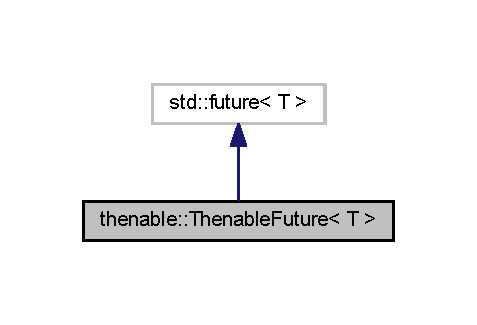
\includegraphics[width=229pt]{classthenable_1_1_thenable_future__inherit__graph}
\end{center}
\end{figure}


Collaboration diagram for thenable\+:\+:Thenable\+Future$<$ T $>$\+:\nopagebreak
\begin{figure}[H]
\begin{center}
\leavevmode
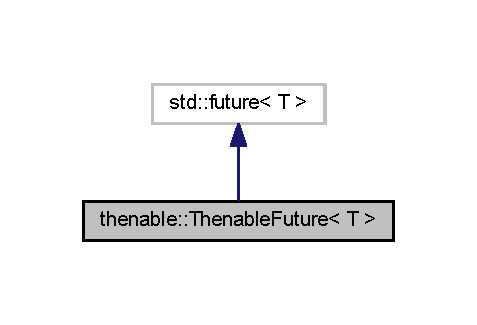
\includegraphics[width=229pt]{classthenable_1_1_thenable_future__coll__graph}
\end{center}
\end{figure}
\subsection*{Public Member Functions}
\begin{DoxyCompactItemize}
\item 
constexpr \hyperlink{classthenable_1_1_thenable_future_a0f196bb64cb0eef8413ecb9e3b399888}{Thenable\+Future} () noexcept
\item 
\hyperlink{classthenable_1_1_thenable_future_a2deca6d5d353e9f65cb14a0d39ab7918}{Thenable\+Future} (std\+::future$<$ T $>$ \&\&f) noexcept
\item 
\hyperlink{classthenable_1_1_thenable_future_afeb709673aa7f3d35dcdad52d4877204}{Thenable\+Future} (\hyperlink{classthenable_1_1_thenable_future}{Thenable\+Future} \&\&f) noexcept
\item 
\hyperlink{classthenable_1_1_thenable_future_a904bc02554b787135b30980d77229e93}{Thenable\+Future} (const \hyperlink{classthenable_1_1_thenable_future}{Thenable\+Future} \&)=delete
\item 
constexpr \hyperlink{classthenable_1_1_thenable_future_ab7fcb7739b5da68d1979138d577db382}{operator std\+::future$<$ T $>$ \&} ()
\item 
constexpr \hyperlink{classthenable_1_1_thenable_future_a6ee994e82bc2e8bb55417a7d3487e549}{operator std\+::future$<$ T $>$ \&\&} ()
\item 
\hyperlink{classthenable_1_1_thenable_future}{Thenable\+Future} \& \hyperlink{classthenable_1_1_thenable_future_a9f0a69b2fa5a4f63596ab4604ba6c028}{operator=} (const \hyperlink{classthenable_1_1_thenable_future}{Thenable\+Future} \&)=delete
\item 
\hyperlink{classthenable_1_1_thenable_shared_future}{Thenable\+Shared\+Future}$<$ T $>$ \hyperlink{classthenable_1_1_thenable_future_a2455963ef10abab0b99003a978cc547d}{share\+\_\+thenable} ()
\item 
{\footnotesize template$<$typename Functor , typename Launch\+Policy  = std\+::launch$>$ }\\\hyperlink{classthenable_1_1_thenable_future}{Thenable\+Future}$<$ \hyperlink{namespacethenable_a1ecf08d6ad8b8688d7b4df047b5feaae}{implicit\+\_\+result\+\_\+of}$<$ Functor, std\+::future$<$ T $>$ $>$ $>$ \hyperlink{classthenable_1_1_thenable_future_a6b284c9a8433018ee39906c0e4922dba}{then} (Functor \&\&f, Launch\+Policy policy=\hyperlink{namespacethenable_a55a20a452e9ba9c0eff946d9b8636f06}{default\+\_\+policy})
\end{DoxyCompactItemize}


\subsection{Detailed Description}
\subsubsection*{template$<$typename T$>$\\*
class thenable\+::\+Thenable\+Future$<$ T $>$}



Definition at line 54 of file thenable.\+hpp.



\subsection{Constructor \& Destructor Documentation}
\index{thenable\+::\+Thenable\+Future@{thenable\+::\+Thenable\+Future}!Thenable\+Future@{Thenable\+Future}}
\index{Thenable\+Future@{Thenable\+Future}!thenable\+::\+Thenable\+Future@{thenable\+::\+Thenable\+Future}}
\subsubsection[{\texorpdfstring{Thenable\+Future() noexcept}{ThenableFuture() noexcept}}]{\setlength{\rightskip}{0pt plus 5cm}template$<$typename T$>$ constexpr {\bf thenable\+::\+Thenable\+Future}$<$ T $>$\+::{\bf Thenable\+Future} (
\begin{DoxyParamCaption}
{}
\end{DoxyParamCaption}
)\hspace{0.3cm}{\ttfamily [inline]}, {\ttfamily [noexcept]}}\hypertarget{classthenable_1_1_thenable_future_a0f196bb64cb0eef8413ecb9e3b399888}{}\label{classthenable_1_1_thenable_future_a0f196bb64cb0eef8413ecb9e3b399888}


Definition at line 701 of file thenable.\+hpp.

\index{thenable\+::\+Thenable\+Future@{thenable\+::\+Thenable\+Future}!Thenable\+Future@{Thenable\+Future}}
\index{Thenable\+Future@{Thenable\+Future}!thenable\+::\+Thenable\+Future@{thenable\+::\+Thenable\+Future}}
\subsubsection[{\texorpdfstring{Thenable\+Future(std\+::future$<$ T $>$ \&\&f) noexcept}{ThenableFuture(std::future< T > &&f) noexcept}}]{\setlength{\rightskip}{0pt plus 5cm}template$<$typename T$>$ {\bf thenable\+::\+Thenable\+Future}$<$ T $>$\+::{\bf Thenable\+Future} (
\begin{DoxyParamCaption}
\item[{std\+::future$<$ T $>$ \&\&}]{f}
\end{DoxyParamCaption}
)\hspace{0.3cm}{\ttfamily [inline]}, {\ttfamily [noexcept]}}\hypertarget{classthenable_1_1_thenable_future_a2deca6d5d353e9f65cb14a0d39ab7918}{}\label{classthenable_1_1_thenable_future_a2deca6d5d353e9f65cb14a0d39ab7918}


Definition at line 703 of file thenable.\+hpp.

\index{thenable\+::\+Thenable\+Future@{thenable\+::\+Thenable\+Future}!Thenable\+Future@{Thenable\+Future}}
\index{Thenable\+Future@{Thenable\+Future}!thenable\+::\+Thenable\+Future@{thenable\+::\+Thenable\+Future}}
\subsubsection[{\texorpdfstring{Thenable\+Future(\+Thenable\+Future \&\&f) noexcept}{ThenableFuture(ThenableFuture &&f) noexcept}}]{\setlength{\rightskip}{0pt plus 5cm}template$<$typename T$>$ {\bf thenable\+::\+Thenable\+Future}$<$ T $>$\+::{\bf Thenable\+Future} (
\begin{DoxyParamCaption}
\item[{{\bf Thenable\+Future}$<$ T $>$ \&\&}]{f}
\end{DoxyParamCaption}
)\hspace{0.3cm}{\ttfamily [inline]}, {\ttfamily [noexcept]}}\hypertarget{classthenable_1_1_thenable_future_afeb709673aa7f3d35dcdad52d4877204}{}\label{classthenable_1_1_thenable_future_afeb709673aa7f3d35dcdad52d4877204}


Definition at line 705 of file thenable.\+hpp.

\index{thenable\+::\+Thenable\+Future@{thenable\+::\+Thenable\+Future}!Thenable\+Future@{Thenable\+Future}}
\index{Thenable\+Future@{Thenable\+Future}!thenable\+::\+Thenable\+Future@{thenable\+::\+Thenable\+Future}}
\subsubsection[{\texorpdfstring{Thenable\+Future(const Thenable\+Future \&)=delete}{ThenableFuture(const ThenableFuture &)=delete}}]{\setlength{\rightskip}{0pt plus 5cm}template$<$typename T$>$ {\bf thenable\+::\+Thenable\+Future}$<$ T $>$\+::{\bf Thenable\+Future} (
\begin{DoxyParamCaption}
\item[{const {\bf Thenable\+Future}$<$ T $>$ \&}]{}
\end{DoxyParamCaption}
)\hspace{0.3cm}{\ttfamily [delete]}}\hypertarget{classthenable_1_1_thenable_future_a904bc02554b787135b30980d77229e93}{}\label{classthenable_1_1_thenable_future_a904bc02554b787135b30980d77229e93}


\subsection{Member Function Documentation}
\index{thenable\+::\+Thenable\+Future@{thenable\+::\+Thenable\+Future}!operator std\+::future$<$ T $>$ \&@{operator std\+::future$<$ T $>$ \&}}
\index{operator std\+::future$<$ T $>$ \&@{operator std\+::future$<$ T $>$ \&}!thenable\+::\+Thenable\+Future@{thenable\+::\+Thenable\+Future}}
\subsubsection[{\texorpdfstring{operator std\+::future$<$ T $>$ \&()}{operator std::future< T > &()}}]{\setlength{\rightskip}{0pt plus 5cm}template$<$typename T$>$ constexpr {\bf thenable\+::\+Thenable\+Future}$<$ T $>$\+::operator std\+::future$<$ T $>$ \& (
\begin{DoxyParamCaption}
{}
\end{DoxyParamCaption}
)\hspace{0.3cm}{\ttfamily [inline]}}\hypertarget{classthenable_1_1_thenable_future_ab7fcb7739b5da68d1979138d577db382}{}\label{classthenable_1_1_thenable_future_ab7fcb7739b5da68d1979138d577db382}


Definition at line 711 of file thenable.\+hpp.

\index{thenable\+::\+Thenable\+Future@{thenable\+::\+Thenable\+Future}!operator std\+::future$<$ T $>$ \&\&@{operator std\+::future$<$ T $>$ \&\&}}
\index{operator std\+::future$<$ T $>$ \&\&@{operator std\+::future$<$ T $>$ \&\&}!thenable\+::\+Thenable\+Future@{thenable\+::\+Thenable\+Future}}
\subsubsection[{\texorpdfstring{operator std\+::future$<$ T $>$ \&\&()}{operator std::future< T > &&()}}]{\setlength{\rightskip}{0pt plus 5cm}template$<$typename T$>$ constexpr {\bf thenable\+::\+Thenable\+Future}$<$ T $>$\+::operator std\+::future$<$ T $>$ \&\& (
\begin{DoxyParamCaption}
{}
\end{DoxyParamCaption}
)\hspace{0.3cm}{\ttfamily [inline]}}\hypertarget{classthenable_1_1_thenable_future_a6ee994e82bc2e8bb55417a7d3487e549}{}\label{classthenable_1_1_thenable_future_a6ee994e82bc2e8bb55417a7d3487e549}


Definition at line 715 of file thenable.\+hpp.

\index{thenable\+::\+Thenable\+Future@{thenable\+::\+Thenable\+Future}!operator=@{operator=}}
\index{operator=@{operator=}!thenable\+::\+Thenable\+Future@{thenable\+::\+Thenable\+Future}}
\subsubsection[{\texorpdfstring{operator=(const Thenable\+Future \&)=delete}{operator=(const ThenableFuture &)=delete}}]{\setlength{\rightskip}{0pt plus 5cm}template$<$typename T$>$ {\bf Thenable\+Future}\& {\bf thenable\+::\+Thenable\+Future}$<$ T $>$\+::operator= (
\begin{DoxyParamCaption}
\item[{const {\bf Thenable\+Future}$<$ T $>$ \&}]{}
\end{DoxyParamCaption}
)\hspace{0.3cm}{\ttfamily [delete]}}\hypertarget{classthenable_1_1_thenable_future_a9f0a69b2fa5a4f63596ab4604ba6c028}{}\label{classthenable_1_1_thenable_future_a9f0a69b2fa5a4f63596ab4604ba6c028}
\index{thenable\+::\+Thenable\+Future@{thenable\+::\+Thenable\+Future}!share\+\_\+thenable@{share\+\_\+thenable}}
\index{share\+\_\+thenable@{share\+\_\+thenable}!thenable\+::\+Thenable\+Future@{thenable\+::\+Thenable\+Future}}
\subsubsection[{\texorpdfstring{share\+\_\+thenable()}{share_thenable()}}]{\setlength{\rightskip}{0pt plus 5cm}template$<$typename T$>$ {\bf Thenable\+Shared\+Future}$<$T$>$ {\bf thenable\+::\+Thenable\+Future}$<$ T $>$\+::share\+\_\+thenable (
\begin{DoxyParamCaption}
{}
\end{DoxyParamCaption}
)\hspace{0.3cm}{\ttfamily [inline]}}\hypertarget{classthenable_1_1_thenable_future_a2455963ef10abab0b99003a978cc547d}{}\label{classthenable_1_1_thenable_future_a2455963ef10abab0b99003a978cc547d}


Definition at line 724 of file thenable.\+hpp.

\index{thenable\+::\+Thenable\+Future@{thenable\+::\+Thenable\+Future}!then@{then}}
\index{then@{then}!thenable\+::\+Thenable\+Future@{thenable\+::\+Thenable\+Future}}
\subsubsection[{\texorpdfstring{then(\+Functor \&\&f, Launch\+Policy policy=default\+\_\+policy)}{then(Functor &&f, LaunchPolicy policy=default_policy)}}]{\setlength{\rightskip}{0pt plus 5cm}template$<$typename T$>$ template$<$typename Functor , typename Launch\+Policy  = std\+::launch$>$ {\bf Thenable\+Future}$<${\bf implicit\+\_\+result\+\_\+of}$<$Functor, std\+::future$<$T$>$ $>$ $>$ {\bf thenable\+::\+Thenable\+Future}$<$ T $>$\+::then (
\begin{DoxyParamCaption}
\item[{Functor \&\&}]{f, }
\item[{Launch\+Policy}]{policy = {\ttfamily {\bf default\+\_\+policy}}}
\end{DoxyParamCaption}
)\hspace{0.3cm}{\ttfamily [inline]}}\hypertarget{classthenable_1_1_thenable_future_a6b284c9a8433018ee39906c0e4922dba}{}\label{classthenable_1_1_thenable_future_a6b284c9a8433018ee39906c0e4922dba}


Definition at line 720 of file thenable.\+hpp.



References thenable\+::then2().



The documentation for this class was generated from the following file\+:\begin{DoxyCompactItemize}
\item 
include/thenable/\hyperlink{thenable_8hpp}{thenable.\+hpp}\end{DoxyCompactItemize}

\hypertarget{classthenable_1_1_thenable_promise}{}\section{thenable\+:\+:Thenable\+Promise$<$ T $>$ Class Template Reference}
\label{classthenable_1_1_thenable_promise}\index{thenable\+::\+Thenable\+Promise$<$ T $>$@{thenable\+::\+Thenable\+Promise$<$ T $>$}}


{\ttfamily \#include $<$thenable.\+hpp$>$}



Inheritance diagram for thenable\+:\+:Thenable\+Promise$<$ T $>$\+:\nopagebreak
\begin{figure}[H]
\begin{center}
\leavevmode
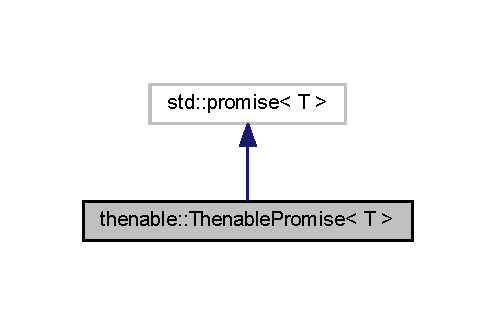
\includegraphics[width=238pt]{classthenable_1_1_thenable_promise__inherit__graph}
\end{center}
\end{figure}


Collaboration diagram for thenable\+:\+:Thenable\+Promise$<$ T $>$\+:\nopagebreak
\begin{figure}[H]
\begin{center}
\leavevmode
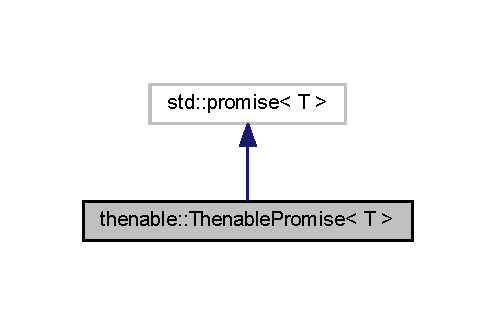
\includegraphics[width=238pt]{classthenable_1_1_thenable_promise__coll__graph}
\end{center}
\end{figure}
\subsection*{Public Member Functions}
\begin{DoxyCompactItemize}
\item 
\hyperlink{classthenable_1_1_thenable_promise_a5dcdc4a9487131b5dd96e084fafb6de6}{Thenable\+Promise} ()
\item 
\hyperlink{classthenable_1_1_thenable_promise_ad25a92a963b5fbd064e378779a5c9bfe}{Thenable\+Promise} (std\+::promise$<$ T $>$ \&\&p)
\item 
\hyperlink{classthenable_1_1_thenable_promise_a9d850b76b46dfb04943553fba4d97323}{Thenable\+Promise} (\hyperlink{classthenable_1_1_thenable_promise}{Thenable\+Promise} \&\&p)
\item 
\hyperlink{classthenable_1_1_thenable_promise_aab4dbabc0987e35017c21026bd995559}{Thenable\+Promise} (const \hyperlink{classthenable_1_1_thenable_promise}{Thenable\+Promise} \&)=delete
\item 
\hyperlink{classthenable_1_1_thenable_future}{Thenable\+Future}$<$ T $>$ \hyperlink{classthenable_1_1_thenable_promise_ae65833002d25ebac014ce36fe945aeca}{get\+\_\+thenable\+\_\+future} ()
\item 
constexpr \hyperlink{classthenable_1_1_thenable_promise_a7245d63eb75cb17f38c8c48467129b54}{operator std\+::promise$<$ T $>$ \&} () noexcept
\item 
constexpr \hyperlink{classthenable_1_1_thenable_promise_a78ab6b269bcca9721b1be918a4ba64d6}{operator std\+::promise$<$ T $>$ \&\&} () noexcept
\item 
\hyperlink{classthenable_1_1_thenable_promise}{Thenable\+Promise} \& \hyperlink{classthenable_1_1_thenable_promise_a7a7ab14665d602c6ccae9e7a97a2005e}{operator=} (const \hyperlink{classthenable_1_1_thenable_promise}{Thenable\+Promise} \&)=delete
\item 
{\footnotesize template$<$typename Functor , typename Launch\+Policy  = std\+::launch$>$ }\\\hyperlink{classthenable_1_1_thenable_future}{Thenable\+Future}$<$ \hyperlink{namespacethenable_a1ecf08d6ad8b8688d7b4df047b5feaae}{implicit\+\_\+result\+\_\+of}$<$ Functor, std\+::future$<$ T $>$ $>$ $>$ \hyperlink{classthenable_1_1_thenable_promise_a236d39e15180107acb51173760f98510}{then} (Functor \&\&f, Launch\+Policy policy=\hyperlink{namespacethenable_a55a20a452e9ba9c0eff946d9b8636f06}{default\+\_\+policy})
\end{DoxyCompactItemize}


\subsection{Detailed Description}
\subsubsection*{template$<$typename T$>$\\*
class thenable\+::\+Thenable\+Promise$<$ T $>$}



Definition at line 60 of file thenable.\+hpp.



\subsection{Constructor \& Destructor Documentation}
\index{thenable\+::\+Thenable\+Promise@{thenable\+::\+Thenable\+Promise}!Thenable\+Promise@{Thenable\+Promise}}
\index{Thenable\+Promise@{Thenable\+Promise}!thenable\+::\+Thenable\+Promise@{thenable\+::\+Thenable\+Promise}}
\subsubsection[{\texorpdfstring{Thenable\+Promise()}{ThenablePromise()}}]{\setlength{\rightskip}{0pt plus 5cm}template$<$typename T$>$ {\bf thenable\+::\+Thenable\+Promise}$<$ T $>$\+::{\bf Thenable\+Promise} (
\begin{DoxyParamCaption}
{}
\end{DoxyParamCaption}
)\hspace{0.3cm}{\ttfamily [inline]}}\hypertarget{classthenable_1_1_thenable_promise_a5dcdc4a9487131b5dd96e084fafb6de6}{}\label{classthenable_1_1_thenable_promise_a5dcdc4a9487131b5dd96e084fafb6de6}


Definition at line 665 of file thenable.\+hpp.

\index{thenable\+::\+Thenable\+Promise@{thenable\+::\+Thenable\+Promise}!Thenable\+Promise@{Thenable\+Promise}}
\index{Thenable\+Promise@{Thenable\+Promise}!thenable\+::\+Thenable\+Promise@{thenable\+::\+Thenable\+Promise}}
\subsubsection[{\texorpdfstring{Thenable\+Promise(std\+::promise$<$ T $>$ \&\&p)}{ThenablePromise(std::promise< T > &&p)}}]{\setlength{\rightskip}{0pt plus 5cm}template$<$typename T$>$ {\bf thenable\+::\+Thenable\+Promise}$<$ T $>$\+::{\bf Thenable\+Promise} (
\begin{DoxyParamCaption}
\item[{std\+::promise$<$ T $>$ \&\&}]{p}
\end{DoxyParamCaption}
)\hspace{0.3cm}{\ttfamily [inline]}}\hypertarget{classthenable_1_1_thenable_promise_ad25a92a963b5fbd064e378779a5c9bfe}{}\label{classthenable_1_1_thenable_promise_ad25a92a963b5fbd064e378779a5c9bfe}


Definition at line 667 of file thenable.\+hpp.

\index{thenable\+::\+Thenable\+Promise@{thenable\+::\+Thenable\+Promise}!Thenable\+Promise@{Thenable\+Promise}}
\index{Thenable\+Promise@{Thenable\+Promise}!thenable\+::\+Thenable\+Promise@{thenable\+::\+Thenable\+Promise}}
\subsubsection[{\texorpdfstring{Thenable\+Promise(\+Thenable\+Promise \&\&p)}{ThenablePromise(ThenablePromise &&p)}}]{\setlength{\rightskip}{0pt plus 5cm}template$<$typename T$>$ {\bf thenable\+::\+Thenable\+Promise}$<$ T $>$\+::{\bf Thenable\+Promise} (
\begin{DoxyParamCaption}
\item[{{\bf Thenable\+Promise}$<$ T $>$ \&\&}]{p}
\end{DoxyParamCaption}
)\hspace{0.3cm}{\ttfamily [inline]}}\hypertarget{classthenable_1_1_thenable_promise_a9d850b76b46dfb04943553fba4d97323}{}\label{classthenable_1_1_thenable_promise_a9d850b76b46dfb04943553fba4d97323}


Definition at line 669 of file thenable.\+hpp.

\index{thenable\+::\+Thenable\+Promise@{thenable\+::\+Thenable\+Promise}!Thenable\+Promise@{Thenable\+Promise}}
\index{Thenable\+Promise@{Thenable\+Promise}!thenable\+::\+Thenable\+Promise@{thenable\+::\+Thenable\+Promise}}
\subsubsection[{\texorpdfstring{Thenable\+Promise(const Thenable\+Promise \&)=delete}{ThenablePromise(const ThenablePromise &)=delete}}]{\setlength{\rightskip}{0pt plus 5cm}template$<$typename T$>$ {\bf thenable\+::\+Thenable\+Promise}$<$ T $>$\+::{\bf Thenable\+Promise} (
\begin{DoxyParamCaption}
\item[{const {\bf Thenable\+Promise}$<$ T $>$ \&}]{}
\end{DoxyParamCaption}
)\hspace{0.3cm}{\ttfamily [delete]}}\hypertarget{classthenable_1_1_thenable_promise_aab4dbabc0987e35017c21026bd995559}{}\label{classthenable_1_1_thenable_promise_aab4dbabc0987e35017c21026bd995559}


\subsection{Member Function Documentation}
\index{thenable\+::\+Thenable\+Promise@{thenable\+::\+Thenable\+Promise}!get\+\_\+thenable\+\_\+future@{get\+\_\+thenable\+\_\+future}}
\index{get\+\_\+thenable\+\_\+future@{get\+\_\+thenable\+\_\+future}!thenable\+::\+Thenable\+Promise@{thenable\+::\+Thenable\+Promise}}
\subsubsection[{\texorpdfstring{get\+\_\+thenable\+\_\+future()}{get_thenable_future()}}]{\setlength{\rightskip}{0pt plus 5cm}template$<$typename T$>$ {\bf Thenable\+Future}$<$T$>$ {\bf thenable\+::\+Thenable\+Promise}$<$ T $>$\+::get\+\_\+thenable\+\_\+future (
\begin{DoxyParamCaption}
{}
\end{DoxyParamCaption}
)\hspace{0.3cm}{\ttfamily [inline]}}\hypertarget{classthenable_1_1_thenable_promise_ae65833002d25ebac014ce36fe945aeca}{}\label{classthenable_1_1_thenable_promise_ae65833002d25ebac014ce36fe945aeca}


Definition at line 683 of file thenable.\+hpp.

\index{thenable\+::\+Thenable\+Promise@{thenable\+::\+Thenable\+Promise}!operator std\+::promise$<$ T $>$ \&@{operator std\+::promise$<$ T $>$ \&}}
\index{operator std\+::promise$<$ T $>$ \&@{operator std\+::promise$<$ T $>$ \&}!thenable\+::\+Thenable\+Promise@{thenable\+::\+Thenable\+Promise}}
\subsubsection[{\texorpdfstring{operator std\+::promise$<$ T $>$ \&() noexcept}{operator std::promise< T > &() noexcept}}]{\setlength{\rightskip}{0pt plus 5cm}template$<$typename T$>$ constexpr {\bf thenable\+::\+Thenable\+Promise}$<$ T $>$\+::operator std\+::promise$<$ T $>$ \& (
\begin{DoxyParamCaption}
{}
\end{DoxyParamCaption}
)\hspace{0.3cm}{\ttfamily [inline]}, {\ttfamily [noexcept]}}\hypertarget{classthenable_1_1_thenable_promise_a7245d63eb75cb17f38c8c48467129b54}{}\label{classthenable_1_1_thenable_promise_a7245d63eb75cb17f38c8c48467129b54}


Definition at line 675 of file thenable.\+hpp.

\index{thenable\+::\+Thenable\+Promise@{thenable\+::\+Thenable\+Promise}!operator std\+::promise$<$ T $>$ \&\&@{operator std\+::promise$<$ T $>$ \&\&}}
\index{operator std\+::promise$<$ T $>$ \&\&@{operator std\+::promise$<$ T $>$ \&\&}!thenable\+::\+Thenable\+Promise@{thenable\+::\+Thenable\+Promise}}
\subsubsection[{\texorpdfstring{operator std\+::promise$<$ T $>$ \&\&() noexcept}{operator std::promise< T > &&() noexcept}}]{\setlength{\rightskip}{0pt plus 5cm}template$<$typename T$>$ constexpr {\bf thenable\+::\+Thenable\+Promise}$<$ T $>$\+::operator std\+::promise$<$ T $>$ \&\& (
\begin{DoxyParamCaption}
{}
\end{DoxyParamCaption}
)\hspace{0.3cm}{\ttfamily [inline]}, {\ttfamily [noexcept]}}\hypertarget{classthenable_1_1_thenable_promise_a78ab6b269bcca9721b1be918a4ba64d6}{}\label{classthenable_1_1_thenable_promise_a78ab6b269bcca9721b1be918a4ba64d6}


Definition at line 679 of file thenable.\+hpp.

\index{thenable\+::\+Thenable\+Promise@{thenable\+::\+Thenable\+Promise}!operator=@{operator=}}
\index{operator=@{operator=}!thenable\+::\+Thenable\+Promise@{thenable\+::\+Thenable\+Promise}}
\subsubsection[{\texorpdfstring{operator=(const Thenable\+Promise \&)=delete}{operator=(const ThenablePromise &)=delete}}]{\setlength{\rightskip}{0pt plus 5cm}template$<$typename T$>$ {\bf Thenable\+Promise}\& {\bf thenable\+::\+Thenable\+Promise}$<$ T $>$\+::operator= (
\begin{DoxyParamCaption}
\item[{const {\bf Thenable\+Promise}$<$ T $>$ \&}]{}
\end{DoxyParamCaption}
)\hspace{0.3cm}{\ttfamily [delete]}}\hypertarget{classthenable_1_1_thenable_promise_a7a7ab14665d602c6ccae9e7a97a2005e}{}\label{classthenable_1_1_thenable_promise_a7a7ab14665d602c6ccae9e7a97a2005e}
\index{thenable\+::\+Thenable\+Promise@{thenable\+::\+Thenable\+Promise}!then@{then}}
\index{then@{then}!thenable\+::\+Thenable\+Promise@{thenable\+::\+Thenable\+Promise}}
\subsubsection[{\texorpdfstring{then(\+Functor \&\&f, Launch\+Policy policy=default\+\_\+policy)}{then(Functor &&f, LaunchPolicy policy=default_policy)}}]{\setlength{\rightskip}{0pt plus 5cm}template$<$typename T$>$ template$<$typename Functor , typename Launch\+Policy  = std\+::launch$>$ {\bf Thenable\+Future}$<${\bf implicit\+\_\+result\+\_\+of}$<$Functor, std\+::future$<$T$>$ $>$ $>$ {\bf thenable\+::\+Thenable\+Promise}$<$ T $>$\+::then (
\begin{DoxyParamCaption}
\item[{Functor \&\&}]{f, }
\item[{Launch\+Policy}]{policy = {\ttfamily {\bf default\+\_\+policy}}}
\end{DoxyParamCaption}
)\hspace{0.3cm}{\ttfamily [inline]}}\hypertarget{classthenable_1_1_thenable_promise_a236d39e15180107acb51173760f98510}{}\label{classthenable_1_1_thenable_promise_a236d39e15180107acb51173760f98510}


Definition at line 688 of file thenable.\+hpp.



References thenable\+::then2().



The documentation for this class was generated from the following file\+:\begin{DoxyCompactItemize}
\item 
include/thenable/\hyperlink{thenable_8hpp}{thenable.\+hpp}\end{DoxyCompactItemize}

\hypertarget{classthenable_1_1_thenable_shared_future}{}\section{thenable\+:\+:Thenable\+Shared\+Future$<$ T $>$ Class Template Reference}
\label{classthenable_1_1_thenable_shared_future}\index{thenable\+::\+Thenable\+Shared\+Future$<$ T $>$@{thenable\+::\+Thenable\+Shared\+Future$<$ T $>$}}


{\ttfamily \#include $<$thenable.\+hpp$>$}



Inheritance diagram for thenable\+:\+:Thenable\+Shared\+Future$<$ T $>$\+:\nopagebreak
\begin{figure}[H]
\begin{center}
\leavevmode
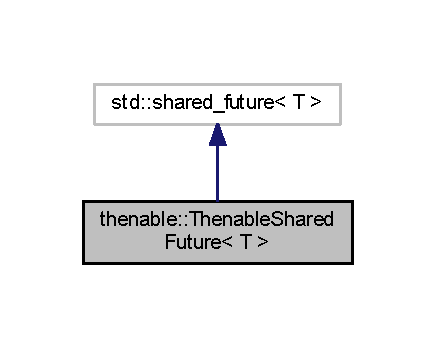
\includegraphics[width=209pt]{classthenable_1_1_thenable_shared_future__inherit__graph}
\end{center}
\end{figure}


Collaboration diagram for thenable\+:\+:Thenable\+Shared\+Future$<$ T $>$\+:\nopagebreak
\begin{figure}[H]
\begin{center}
\leavevmode
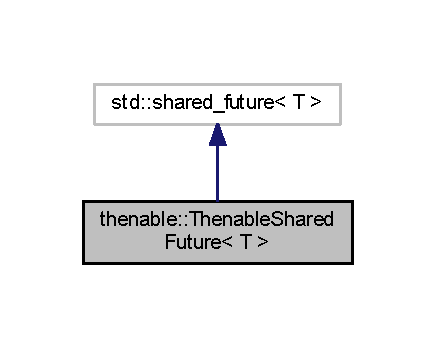
\includegraphics[width=209pt]{classthenable_1_1_thenable_shared_future__coll__graph}
\end{center}
\end{figure}
\subsection*{Public Member Functions}
\begin{DoxyCompactItemize}
\item 
constexpr \hyperlink{classthenable_1_1_thenable_shared_future_a44430012855789b78afce4dce6fa27fe}{Thenable\+Shared\+Future} () noexcept
\item 
\hyperlink{classthenable_1_1_thenable_shared_future_a754294e043ca43dd8b6f4cb1a592072f}{Thenable\+Shared\+Future} (const std\+::shared\+\_\+future$<$ T $>$ \&f) noexcept
\item 
\hyperlink{classthenable_1_1_thenable_shared_future_a163f4c1e38e309eb307e6d92f05ca64c}{Thenable\+Shared\+Future} (const \hyperlink{classthenable_1_1_thenable_shared_future}{Thenable\+Shared\+Future} \&f) noexcept
\item 
\hyperlink{classthenable_1_1_thenable_shared_future_a595a43fe55c970694c0b9af5eb52d2ac}{Thenable\+Shared\+Future} (std\+::future$<$ T $>$ \&\&f) noexcept
\item 
\hyperlink{classthenable_1_1_thenable_shared_future_a0da9026f90c669869bcbcc4827df2d0c}{Thenable\+Shared\+Future} (\hyperlink{classthenable_1_1_thenable_future}{Thenable\+Future}$<$ T $>$ \&\&f) noexcept
\item 
\hyperlink{classthenable_1_1_thenable_shared_future_a0a6f2dc98dcbb177c590ef49191a511a}{Thenable\+Shared\+Future} (std\+::shared\+\_\+future$<$ T $>$ \&\&f) noexcept
\item 
\hyperlink{classthenable_1_1_thenable_shared_future_acbbd8fe47ccd6a8a5512d0e725dd6fac}{Thenable\+Shared\+Future} (\hyperlink{classthenable_1_1_thenable_shared_future}{Thenable\+Shared\+Future} \&\&f) noexcept
\item 
constexpr \hyperlink{classthenable_1_1_thenable_shared_future_ac0fd0a51c6c8e4fd434c8942f2e0a34a}{operator std\+::shared\+\_\+future$<$ T $>$ \&} ()
\item 
constexpr \hyperlink{classthenable_1_1_thenable_shared_future_a4805c90240683e4883c31754569b0f05}{operator std\+::shared\+\_\+future$<$ T $>$ \&\&} ()
\item 
{\footnotesize template$<$typename Functor , typename Launch\+Policy  = std\+::launch$>$ }\\\hyperlink{classthenable_1_1_thenable_future}{Thenable\+Future}$<$ \hyperlink{namespacethenable_a1ecf08d6ad8b8688d7b4df047b5feaae}{implicit\+\_\+result\+\_\+of}$<$ Functor, std\+::shared\+\_\+future$<$ T $>$ $>$ $>$ \hyperlink{classthenable_1_1_thenable_shared_future_a002763be3a45b4c038f687b425c227f8}{then} (Functor \&\&f, Launch\+Policy policy=\hyperlink{namespacethenable_a55a20a452e9ba9c0eff946d9b8636f06}{default\+\_\+policy})
\end{DoxyCompactItemize}


\subsection{Detailed Description}
\subsubsection*{template$<$typename T$>$\\*
class thenable\+::\+Thenable\+Shared\+Future$<$ T $>$}



Definition at line 57 of file thenable.\+hpp.



\subsection{Constructor \& Destructor Documentation}
\index{thenable\+::\+Thenable\+Shared\+Future@{thenable\+::\+Thenable\+Shared\+Future}!Thenable\+Shared\+Future@{Thenable\+Shared\+Future}}
\index{Thenable\+Shared\+Future@{Thenable\+Shared\+Future}!thenable\+::\+Thenable\+Shared\+Future@{thenable\+::\+Thenable\+Shared\+Future}}
\subsubsection[{\texorpdfstring{Thenable\+Shared\+Future() noexcept}{ThenableSharedFuture() noexcept}}]{\setlength{\rightskip}{0pt plus 5cm}template$<$typename T$>$ constexpr {\bf thenable\+::\+Thenable\+Shared\+Future}$<$ T $>$\+::{\bf Thenable\+Shared\+Future} (
\begin{DoxyParamCaption}
{}
\end{DoxyParamCaption}
)\hspace{0.3cm}{\ttfamily [inline]}, {\ttfamily [noexcept]}}\hypertarget{classthenable_1_1_thenable_shared_future_a44430012855789b78afce4dce6fa27fe}{}\label{classthenable_1_1_thenable_shared_future_a44430012855789b78afce4dce6fa27fe}


Definition at line 732 of file thenable.\+hpp.

\index{thenable\+::\+Thenable\+Shared\+Future@{thenable\+::\+Thenable\+Shared\+Future}!Thenable\+Shared\+Future@{Thenable\+Shared\+Future}}
\index{Thenable\+Shared\+Future@{Thenable\+Shared\+Future}!thenable\+::\+Thenable\+Shared\+Future@{thenable\+::\+Thenable\+Shared\+Future}}
\subsubsection[{\texorpdfstring{Thenable\+Shared\+Future(const std\+::shared\+\_\+future$<$ T $>$ \&f) noexcept}{ThenableSharedFuture(const std::shared_future< T > &f) noexcept}}]{\setlength{\rightskip}{0pt plus 5cm}template$<$typename T$>$ {\bf thenable\+::\+Thenable\+Shared\+Future}$<$ T $>$\+::{\bf Thenable\+Shared\+Future} (
\begin{DoxyParamCaption}
\item[{const std\+::shared\+\_\+future$<$ T $>$ \&}]{f}
\end{DoxyParamCaption}
)\hspace{0.3cm}{\ttfamily [inline]}, {\ttfamily [noexcept]}}\hypertarget{classthenable_1_1_thenable_shared_future_a754294e043ca43dd8b6f4cb1a592072f}{}\label{classthenable_1_1_thenable_shared_future_a754294e043ca43dd8b6f4cb1a592072f}


Definition at line 734 of file thenable.\+hpp.

\index{thenable\+::\+Thenable\+Shared\+Future@{thenable\+::\+Thenable\+Shared\+Future}!Thenable\+Shared\+Future@{Thenable\+Shared\+Future}}
\index{Thenable\+Shared\+Future@{Thenable\+Shared\+Future}!thenable\+::\+Thenable\+Shared\+Future@{thenable\+::\+Thenable\+Shared\+Future}}
\subsubsection[{\texorpdfstring{Thenable\+Shared\+Future(const Thenable\+Shared\+Future \&f) noexcept}{ThenableSharedFuture(const ThenableSharedFuture &f) noexcept}}]{\setlength{\rightskip}{0pt plus 5cm}template$<$typename T$>$ {\bf thenable\+::\+Thenable\+Shared\+Future}$<$ T $>$\+::{\bf Thenable\+Shared\+Future} (
\begin{DoxyParamCaption}
\item[{const {\bf Thenable\+Shared\+Future}$<$ T $>$ \&}]{f}
\end{DoxyParamCaption}
)\hspace{0.3cm}{\ttfamily [inline]}, {\ttfamily [noexcept]}}\hypertarget{classthenable_1_1_thenable_shared_future_a163f4c1e38e309eb307e6d92f05ca64c}{}\label{classthenable_1_1_thenable_shared_future_a163f4c1e38e309eb307e6d92f05ca64c}


Definition at line 736 of file thenable.\+hpp.

\index{thenable\+::\+Thenable\+Shared\+Future@{thenable\+::\+Thenable\+Shared\+Future}!Thenable\+Shared\+Future@{Thenable\+Shared\+Future}}
\index{Thenable\+Shared\+Future@{Thenable\+Shared\+Future}!thenable\+::\+Thenable\+Shared\+Future@{thenable\+::\+Thenable\+Shared\+Future}}
\subsubsection[{\texorpdfstring{Thenable\+Shared\+Future(std\+::future$<$ T $>$ \&\&f) noexcept}{ThenableSharedFuture(std::future< T > &&f) noexcept}}]{\setlength{\rightskip}{0pt plus 5cm}template$<$typename T$>$ {\bf thenable\+::\+Thenable\+Shared\+Future}$<$ T $>$\+::{\bf Thenable\+Shared\+Future} (
\begin{DoxyParamCaption}
\item[{std\+::future$<$ T $>$ \&\&}]{f}
\end{DoxyParamCaption}
)\hspace{0.3cm}{\ttfamily [inline]}, {\ttfamily [noexcept]}}\hypertarget{classthenable_1_1_thenable_shared_future_a595a43fe55c970694c0b9af5eb52d2ac}{}\label{classthenable_1_1_thenable_shared_future_a595a43fe55c970694c0b9af5eb52d2ac}


Definition at line 738 of file thenable.\+hpp.

\index{thenable\+::\+Thenable\+Shared\+Future@{thenable\+::\+Thenable\+Shared\+Future}!Thenable\+Shared\+Future@{Thenable\+Shared\+Future}}
\index{Thenable\+Shared\+Future@{Thenable\+Shared\+Future}!thenable\+::\+Thenable\+Shared\+Future@{thenable\+::\+Thenable\+Shared\+Future}}
\subsubsection[{\texorpdfstring{Thenable\+Shared\+Future(\+Thenable\+Future$<$ T $>$ \&\&f) noexcept}{ThenableSharedFuture(ThenableFuture< T > &&f) noexcept}}]{\setlength{\rightskip}{0pt plus 5cm}template$<$typename T$>$ {\bf thenable\+::\+Thenable\+Shared\+Future}$<$ T $>$\+::{\bf Thenable\+Shared\+Future} (
\begin{DoxyParamCaption}
\item[{{\bf Thenable\+Future}$<$ T $>$ \&\&}]{f}
\end{DoxyParamCaption}
)\hspace{0.3cm}{\ttfamily [inline]}, {\ttfamily [noexcept]}}\hypertarget{classthenable_1_1_thenable_shared_future_a0da9026f90c669869bcbcc4827df2d0c}{}\label{classthenable_1_1_thenable_shared_future_a0da9026f90c669869bcbcc4827df2d0c}


Definition at line 740 of file thenable.\+hpp.

\index{thenable\+::\+Thenable\+Shared\+Future@{thenable\+::\+Thenable\+Shared\+Future}!Thenable\+Shared\+Future@{Thenable\+Shared\+Future}}
\index{Thenable\+Shared\+Future@{Thenable\+Shared\+Future}!thenable\+::\+Thenable\+Shared\+Future@{thenable\+::\+Thenable\+Shared\+Future}}
\subsubsection[{\texorpdfstring{Thenable\+Shared\+Future(std\+::shared\+\_\+future$<$ T $>$ \&\&f) noexcept}{ThenableSharedFuture(std::shared_future< T > &&f) noexcept}}]{\setlength{\rightskip}{0pt plus 5cm}template$<$typename T$>$ {\bf thenable\+::\+Thenable\+Shared\+Future}$<$ T $>$\+::{\bf Thenable\+Shared\+Future} (
\begin{DoxyParamCaption}
\item[{std\+::shared\+\_\+future$<$ T $>$ \&\&}]{f}
\end{DoxyParamCaption}
)\hspace{0.3cm}{\ttfamily [inline]}, {\ttfamily [noexcept]}}\hypertarget{classthenable_1_1_thenable_shared_future_a0a6f2dc98dcbb177c590ef49191a511a}{}\label{classthenable_1_1_thenable_shared_future_a0a6f2dc98dcbb177c590ef49191a511a}


Definition at line 742 of file thenable.\+hpp.

\index{thenable\+::\+Thenable\+Shared\+Future@{thenable\+::\+Thenable\+Shared\+Future}!Thenable\+Shared\+Future@{Thenable\+Shared\+Future}}
\index{Thenable\+Shared\+Future@{Thenable\+Shared\+Future}!thenable\+::\+Thenable\+Shared\+Future@{thenable\+::\+Thenable\+Shared\+Future}}
\subsubsection[{\texorpdfstring{Thenable\+Shared\+Future(\+Thenable\+Shared\+Future \&\&f) noexcept}{ThenableSharedFuture(ThenableSharedFuture &&f) noexcept}}]{\setlength{\rightskip}{0pt plus 5cm}template$<$typename T$>$ {\bf thenable\+::\+Thenable\+Shared\+Future}$<$ T $>$\+::{\bf Thenable\+Shared\+Future} (
\begin{DoxyParamCaption}
\item[{{\bf Thenable\+Shared\+Future}$<$ T $>$ \&\&}]{f}
\end{DoxyParamCaption}
)\hspace{0.3cm}{\ttfamily [inline]}, {\ttfamily [noexcept]}}\hypertarget{classthenable_1_1_thenable_shared_future_acbbd8fe47ccd6a8a5512d0e725dd6fac}{}\label{classthenable_1_1_thenable_shared_future_acbbd8fe47ccd6a8a5512d0e725dd6fac}


Definition at line 744 of file thenable.\+hpp.



\subsection{Member Function Documentation}
\index{thenable\+::\+Thenable\+Shared\+Future@{thenable\+::\+Thenable\+Shared\+Future}!operator std\+::shared\+\_\+future$<$ T $>$ \&@{operator std\+::shared\+\_\+future$<$ T $>$ \&}}
\index{operator std\+::shared\+\_\+future$<$ T $>$ \&@{operator std\+::shared\+\_\+future$<$ T $>$ \&}!thenable\+::\+Thenable\+Shared\+Future@{thenable\+::\+Thenable\+Shared\+Future}}
\subsubsection[{\texorpdfstring{operator std\+::shared\+\_\+future$<$ T $>$ \&()}{operator std::shared_future< T > &()}}]{\setlength{\rightskip}{0pt plus 5cm}template$<$typename T$>$ constexpr {\bf thenable\+::\+Thenable\+Shared\+Future}$<$ T $>$\+::operator std\+::shared\+\_\+future$<$ T $>$ \& (
\begin{DoxyParamCaption}
{}
\end{DoxyParamCaption}
)\hspace{0.3cm}{\ttfamily [inline]}}\hypertarget{classthenable_1_1_thenable_shared_future_ac0fd0a51c6c8e4fd434c8942f2e0a34a}{}\label{classthenable_1_1_thenable_shared_future_ac0fd0a51c6c8e4fd434c8942f2e0a34a}


Definition at line 746 of file thenable.\+hpp.

\index{thenable\+::\+Thenable\+Shared\+Future@{thenable\+::\+Thenable\+Shared\+Future}!operator std\+::shared\+\_\+future$<$ T $>$ \&\&@{operator std\+::shared\+\_\+future$<$ T $>$ \&\&}}
\index{operator std\+::shared\+\_\+future$<$ T $>$ \&\&@{operator std\+::shared\+\_\+future$<$ T $>$ \&\&}!thenable\+::\+Thenable\+Shared\+Future@{thenable\+::\+Thenable\+Shared\+Future}}
\subsubsection[{\texorpdfstring{operator std\+::shared\+\_\+future$<$ T $>$ \&\&()}{operator std::shared_future< T > &&()}}]{\setlength{\rightskip}{0pt plus 5cm}template$<$typename T$>$ constexpr {\bf thenable\+::\+Thenable\+Shared\+Future}$<$ T $>$\+::operator std\+::shared\+\_\+future$<$ T $>$ \&\& (
\begin{DoxyParamCaption}
{}
\end{DoxyParamCaption}
)\hspace{0.3cm}{\ttfamily [inline]}}\hypertarget{classthenable_1_1_thenable_shared_future_a4805c90240683e4883c31754569b0f05}{}\label{classthenable_1_1_thenable_shared_future_a4805c90240683e4883c31754569b0f05}


Definition at line 750 of file thenable.\+hpp.

\index{thenable\+::\+Thenable\+Shared\+Future@{thenable\+::\+Thenable\+Shared\+Future}!then@{then}}
\index{then@{then}!thenable\+::\+Thenable\+Shared\+Future@{thenable\+::\+Thenable\+Shared\+Future}}
\subsubsection[{\texorpdfstring{then(\+Functor \&\&f, Launch\+Policy policy=default\+\_\+policy)}{then(Functor &&f, LaunchPolicy policy=default_policy)}}]{\setlength{\rightskip}{0pt plus 5cm}template$<$typename T$>$ template$<$typename Functor , typename Launch\+Policy  = std\+::launch$>$ {\bf Thenable\+Future}$<${\bf implicit\+\_\+result\+\_\+of}$<$Functor, std\+::shared\+\_\+future$<$T$>$ $>$ $>$ {\bf thenable\+::\+Thenable\+Shared\+Future}$<$ T $>$\+::then (
\begin{DoxyParamCaption}
\item[{Functor \&\&}]{f, }
\item[{Launch\+Policy}]{policy = {\ttfamily {\bf default\+\_\+policy}}}
\end{DoxyParamCaption}
)\hspace{0.3cm}{\ttfamily [inline]}}\hypertarget{classthenable_1_1_thenable_shared_future_a002763be3a45b4c038f687b425c227f8}{}\label{classthenable_1_1_thenable_shared_future_a002763be3a45b4c038f687b425c227f8}


Definition at line 755 of file thenable.\+hpp.



References thenable\+::then2().



The documentation for this class was generated from the following file\+:\begin{DoxyCompactItemize}
\item 
include/thenable/\hyperlink{thenable_8hpp}{thenable.\+hpp}\end{DoxyCompactItemize}

\chapter{File Documentation}
\hypertarget{experimental_8hpp}{}\section{include/thenable/experimental.hpp File Reference}
\label{experimental_8hpp}\index{include/thenable/experimental.\+hpp@{include/thenable/experimental.\+hpp}}
{\ttfamily \#include $<$thenable/thenable.\+hpp$>$}\\*
{\ttfamily \#include $<$atomic$>$}\\*
{\ttfamily \#include $<$algorithm$>$}\\*
{\ttfamily \#include $<$utility$>$}\\*
{\ttfamily \#include $<$initializer\+\_\+list$>$}\\*
Include dependency graph for experimental.\+hpp\+:
\nopagebreak
\begin{figure}[H]
\begin{center}
\leavevmode
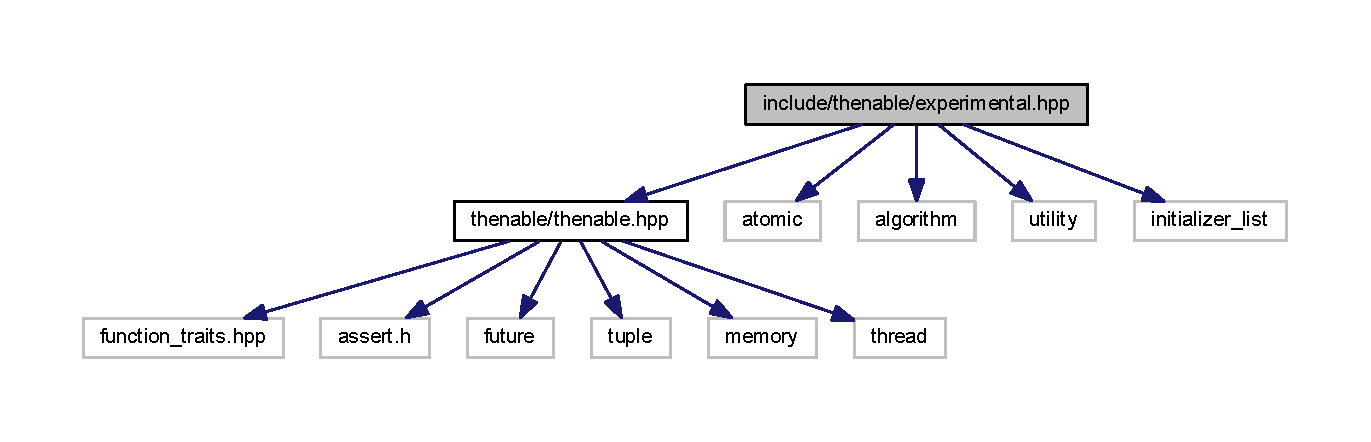
\includegraphics[width=350pt]{experimental_8hpp__incl}
\end{center}
\end{figure}
\subsection*{Namespaces}
\begin{DoxyCompactItemize}
\item 
 \hyperlink{namespacethenable}{thenable}
\item 
 \hyperlink{namespacethenable_1_1experimental}{thenable\+::experimental}
\end{DoxyCompactItemize}

\hypertarget{thenable_8hpp}{}\section{include/thenable/thenable.hpp File Reference}
\label{thenable_8hpp}\index{include/thenable/thenable.\+hpp@{include/thenable/thenable.\+hpp}}
{\ttfamily \#include $<$function\+\_\+traits.\+hpp$>$}\\*
{\ttfamily \#include $<$assert.\+h$>$}\\*
{\ttfamily \#include $<$future$>$}\\*
{\ttfamily \#include $<$tuple$>$}\\*
{\ttfamily \#include $<$memory$>$}\\*
{\ttfamily \#include $<$thread$>$}\\*
Include dependency graph for thenable.\+hpp\+:
\nopagebreak
\begin{figure}[H]
\begin{center}
\leavevmode
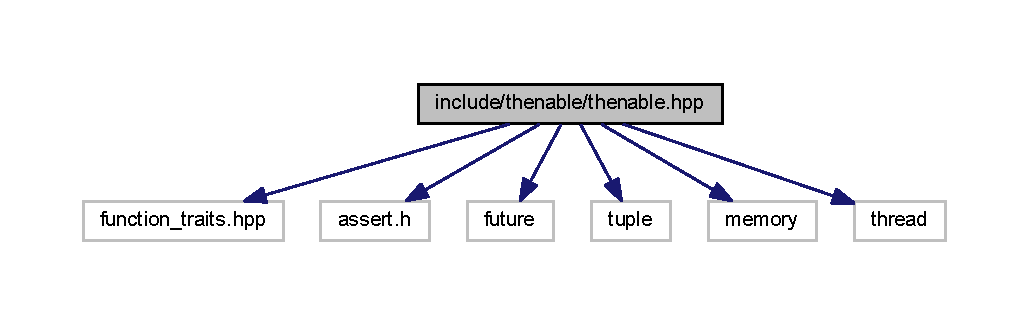
\includegraphics[width=350pt]{thenable_8hpp__incl}
\end{center}
\end{figure}
This graph shows which files directly or indirectly include this file\+:
\nopagebreak
\begin{figure}[H]
\begin{center}
\leavevmode
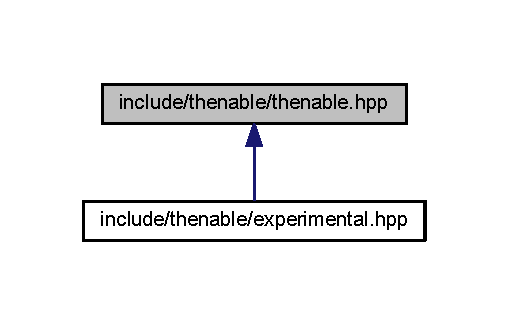
\includegraphics[width=244pt]{thenable_8hpp__dep__incl}
\end{center}
\end{figure}
\subsection*{Classes}
\begin{DoxyCompactItemize}
\item 
class \hyperlink{classthenable_1_1_thenable_future}{thenable\+::\+Thenable\+Future$<$ T $>$}
\item 
class \hyperlink{classthenable_1_1_thenable_future}{thenable\+::\+Thenable\+Future$<$ T $>$}
\item 
class \hyperlink{classthenable_1_1_thenable_promise}{thenable\+::\+Thenable\+Promise$<$ T $>$}
\item 
class \hyperlink{classthenable_1_1_thenable_promise}{thenable\+::\+Thenable\+Promise$<$ T $>$}
\item 
class \hyperlink{classthenable_1_1_thenable_shared_future}{thenable\+::\+Thenable\+Shared\+Future$<$ T $>$}
\item 
class \hyperlink{classthenable_1_1_thenable_shared_future}{thenable\+::\+Thenable\+Shared\+Future$<$ T $>$}
\end{DoxyCompactItemize}
\subsection*{Namespaces}
\begin{DoxyCompactItemize}
\item 
 \hyperlink{namespacethenable}{thenable}
\end{DoxyCompactItemize}
\subsection*{Typedefs}
\begin{DoxyCompactItemize}
\item 
{\footnotesize template$<$typename Functor , typename Future\+Type $>$ }\\using \hyperlink{namespacethenable_a1ecf08d6ad8b8688d7b4df047b5feaae}{thenable\+::implicit\+\_\+result\+\_\+of} = decltype(detail\+::then\+\_\+helper$<$ typename detail\+::get\+\_\+future\+\_\+type$<$ typename std\+::remove\+\_\+reference$<$ Future\+Type $>$\+::type $>$\+::type, Functor $>$\+::dispatch(std\+::forward$<$ Future\+Type $>$(std\+::declval$<$ Future\+Type $>$()), std\+::forward$<$ Functor $>$(std\+::declval$<$ Functor $>$())))
\item 
{\footnotesize template$<$typename Functor $>$ }\\using \hyperlink{namespacethenable_a71ee91c31ba9c80bb2d6f3effe4bae12}{thenable\+::recursive\+\_\+result\+\_\+of} = typename detail\+::recursive\+\_\+get\+\_\+type$<$ typename std\+::result\+\_\+of$<$ Functor()$>$\+::type $>$\+::type
\end{DoxyCompactItemize}
\subsection*{Enumerations}
\begin{DoxyCompactItemize}
\item 
enum \hyperlink{namespacethenable_adf31291b806157ad914943dae5b3c94e}{thenable\+::then\+\_\+launch} \{ \hyperlink{namespacethenable_adf31291b806157ad914943dae5b3c94eab0398fd2e0c78072a48131f810266119}{thenable\+::then\+\_\+launch\+::detached} = 4
 \}
\end{DoxyCompactItemize}
\subsection*{Functions}
\begin{DoxyCompactItemize}
\item 
{\footnotesize template$<$typename... Results$>$ }\\std\+::future$<$ std\+::tuple$<$ Results... $>$ $>$ \hyperlink{namespacethenable_a37ee216d9dc5925d9b29253d2995aa61}{thenable\+::await\+\_\+all} (std\+::tuple$<$ std\+::future$<$ Results $>$... $>$ \&\&results, std\+::launch policy=default\+\_\+policy)
\item 
{\footnotesize template$<$typename... Results$>$ }\\std\+::future$<$ std\+::tuple$<$ Results... $>$ $>$ \hyperlink{namespacethenable_a25eb0856c1e74aa180ab2b0d37313ef2}{thenable\+::await\+\_\+all} (std\+::tuple$<$ std\+::shared\+\_\+future$<$ Results $>$... $>$ \&\&results, std\+::launch policy=default\+\_\+policy)
\item 
{\footnotesize template$<$typename... Results$>$ }\\Thenable\+Future$<$ std\+::tuple$<$ Results... $>$ $>$ \hyperlink{namespacethenable_a8b68e9ecc3341f793b7d5d83546c360c}{thenable\+::await\+\_\+all} (std\+::tuple$<$ Thenable\+Future$<$ Results $>$... $>$ \&\&results, std\+::launch policy=default\+\_\+policy)
\item 
{\footnotesize template$<$typename... Results$>$ }\\Thenable\+Future$<$ std\+::tuple$<$ Results... $>$ $>$ \hyperlink{namespacethenable_aa67b5bd21ea878bcfabf190dc53f3b93}{thenable\+::await\+\_\+all} (std\+::tuple$<$ Thenable\+Shared\+Future$<$ Results $>$... $>$ \&\&results, std\+::launch policy=default\+\_\+policy)
\item 
{\footnotesize template$<$typename... Results$>$ }\\std\+::future$<$ std\+::tuple$<$ Results... $>$ $>$ \hyperlink{namespacethenable_a2b77cbbe1f031af6dbea0797de52894a}{thenable\+::await\+\_\+all} (std\+::tuple$<$ std\+::promise$<$ Results $>$... $>$ \&\&results, std\+::launch policy=default\+\_\+policy)
\item 
{\footnotesize template$<$typename... Results$>$ }\\Thenable\+Future$<$ std\+::tuple$<$ Results... $>$ $>$ \hyperlink{namespacethenable_a80d6c4269437d398a16de61461415242}{thenable\+::await\+\_\+all} (std\+::tuple$<$ Thenable\+Promise$<$ Results $>$... $>$ \&\&results, std\+::launch policy=default\+\_\+policy)
\item 
{\footnotesize template$<$typename... Results$>$ }\\std\+::future$<$ std\+::tuple$<$ Results... $>$ $>$ \hyperlink{namespacethenable_a52de34f95415017a3716c1e7c37ace7f}{thenable\+::await\+\_\+all} (std\+::tuple$<$ std\+::future$<$ Results $>$... $>$ \&\&results, then\+\_\+launch policy)
\item 
{\footnotesize template$<$typename... Results$>$ }\\std\+::future$<$ std\+::tuple$<$ Results... $>$ $>$ \hyperlink{namespacethenable_a7b2baeb104fb7115a97586739f08af1e}{thenable\+::await\+\_\+all} (std\+::tuple$<$ std\+::shared\+\_\+future$<$ Results $>$... $>$ \&\&results, then\+\_\+launch policy)
\item 
{\footnotesize template$<$typename... Results$>$ }\\Thenable\+Future$<$ std\+::tuple$<$ Results... $>$ $>$ \hyperlink{namespacethenable_a7e395690cce41b4b74628f989ca90c9c}{thenable\+::await\+\_\+all} (std\+::tuple$<$ Thenable\+Future$<$ Results $>$... $>$ \&\&results, then\+\_\+launch policy)
\item 
{\footnotesize template$<$typename... Results$>$ }\\Thenable\+Future$<$ std\+::tuple$<$ Results... $>$ $>$ \hyperlink{namespacethenable_af6530bd65e65f6c860e43b5b7ab498a1}{thenable\+::await\+\_\+all} (std\+::tuple$<$ Thenable\+Shared\+Future$<$ Results $>$... $>$ \&\&results, then\+\_\+launch policy)
\item 
{\footnotesize template$<$typename... Results$>$ }\\std\+::future$<$ std\+::tuple$<$ Results... $>$ $>$ \hyperlink{namespacethenable_a35735af341e005998045c5705c8994d9}{thenable\+::await\+\_\+all} (std\+::tuple$<$ std\+::promise$<$ Results $>$... $>$ \&\&results, then\+\_\+launch policy)
\item 
{\footnotesize template$<$typename... Results$>$ }\\Thenable\+Future$<$ std\+::tuple$<$ Results... $>$ $>$ \hyperlink{namespacethenable_a497fff66463a0580dd10977df3e0549a}{thenable\+::await\+\_\+all} (std\+::tuple$<$ Thenable\+Promise$<$ Results $>$... $>$ \&\&results, then\+\_\+launch policy)
\item 
{\footnotesize template$<$typename Functor , typename... Args$>$ }\\std\+::future$<$ typename std\+::result\+\_\+of$<$ Functor(Args...)$>$\+::type $>$ \hyperlink{namespacethenable_aceaaf1439cfecf2aab95b6632aadf579}{thenable\+::defer} (Functor \&\&f, Args \&\&...args)
\item 
{\footnotesize template$<$typename Functor , typename... Args$>$ }\\Thenable\+Future$<$ typename std\+::result\+\_\+of$<$ Functor(Args...)$>$\+::type $>$ \hyperlink{namespacethenable_ad9ad041b2e810ef9b1325657a68a48d7}{thenable\+::defer2} (Functor \&\&f, Args \&\&...args)
\item 
{\footnotesize template$<$typename T  = void, typename Functor , typename Launch\+Policy  = std\+::launch$>$ }\\std\+::future$<$ T $>$ \hyperlink{namespacethenable_af2607b8a2775a7d983793a497aad3904}{thenable\+::make\+\_\+promise} (Functor \&\&, Launch\+Policy=default\+\_\+policy)
\item 
{\footnotesize template$<$typename T  = void, typename Functor , typename Launch\+Policy  = std\+::launch$>$ }\\Thenable\+Future$<$ T $>$ \hyperlink{namespacethenable_a48b432e0694e822676fac2de12263a43}{thenable\+::make\+\_\+promise2} (Functor \&\&, Launch\+Policy=default\+\_\+policy)
\item 
{\footnotesize template$<$typename... Functors$>$ }\\std\+::tuple$<$ std\+::future$<$ recursive\+\_\+result\+\_\+of$<$ Functors $>$ $>$... $>$ \hyperlink{namespacethenable_a95e108dc8790ef2db88424ea3ae46c79}{thenable\+::parallel} (Functors \&\&...fns)
\item 
{\footnotesize template$<$typename... Functors$>$ }\\std\+::tuple$<$ Thenable\+Future$<$ recursive\+\_\+result\+\_\+of$<$ Functors $>$ $>$... $>$ \hyperlink{namespacethenable_a4619a50a59383db8a890cc02d8e44262}{thenable\+::parallel2} (Functors \&\&...fns)
\item 
{\footnotesize template$<$typename... Functors$>$ }\\std\+::tuple$<$ Thenable\+Future$<$ recursive\+\_\+result\+\_\+of$<$ Functors $>$ $>$... $>$ \hyperlink{namespacethenable_ae386feb6dd2b3b1171a9f40f25b57f22}{thenable\+::parallel2\+\_\+n} (size\+\_\+t concurrency, Functors \&\&...fns)
\item 
{\footnotesize template$<$typename... Functors$>$ }\\std\+::tuple$<$ std\+::future$<$ recursive\+\_\+result\+\_\+of$<$ Functors $>$ $>$... $>$ \hyperlink{namespacethenable_ae08454ef27fbe2ce5a3f6b2b008a0bc2}{thenable\+::parallel\+\_\+n} (size\+\_\+t concurrency, Functors \&\&...fns)
\item 
{\footnotesize template$<$typename T , typename Functor $>$ }\\std\+::future$<$ implicit\+\_\+result\+\_\+of$<$ Functor, std\+::future$<$ T $>$ $>$ $>$ \hyperlink{namespacethenable_aa7417767a6d39589457c2569f900e9e8}{thenable\+::then} (std\+::future$<$ T $>$ \&, Functor \&\&, std\+::launch=default\+\_\+policy)
\item 
{\footnotesize template$<$typename T , typename Functor $>$ }\\std\+::future$<$ implicit\+\_\+result\+\_\+of$<$ Functor, std\+::shared\+\_\+future$<$ T $>$ $>$ $>$ \hyperlink{namespacethenable_a591eb14beddb29e6d25591b5f85af87a}{thenable\+::then} (std\+::shared\+\_\+future$<$ T $>$ \&\&, Functor \&\&, std\+::launch=default\+\_\+policy)
\item 
{\footnotesize template$<$typename T , typename Functor $>$ }\\std\+::future$<$ implicit\+\_\+result\+\_\+of$<$ Functor, std\+::shared\+\_\+future$<$ T $>$ $>$ $>$ \hyperlink{namespacethenable_ad47a2c35aefe434a7be8c074b1dda08a}{thenable\+::then} (std\+::shared\+\_\+future$<$ T $>$, Functor \&\&, std\+::launch=default\+\_\+policy)
\item 
{\footnotesize template$<$typename T , typename Functor $>$ }\\std\+::future$<$ implicit\+\_\+result\+\_\+of$<$ Functor, std\+::future$<$ T $>$ $>$ $>$ \hyperlink{namespacethenable_a90ae1a436866f21049d7a00a350eb3db}{thenable\+::then} (std\+::future$<$ T $>$ \&\&, Functor \&\&, std\+::launch=default\+\_\+policy)
\item 
{\footnotesize template$<$typename T , typename Functor $>$ }\\std\+::future$<$ implicit\+\_\+result\+\_\+of$<$ Functor, std\+::future$<$ T $>$ $>$ $>$ \hyperlink{namespacethenable_a5e3ae302e707336194333b10694e1fce}{thenable\+::then} (std\+::promise$<$ T $>$ \&, Functor \&\&, std\+::launch=default\+\_\+policy)
\item 
{\footnotesize template$<$typename T , typename Functor $>$ }\\std\+::future$<$ implicit\+\_\+result\+\_\+of$<$ Functor, std\+::future$<$ T $>$ $>$ $>$ \hyperlink{namespacethenable_ab8091f2d67ec80c1f1df9e8f10ed099f}{thenable\+::then} (std\+::future$<$ T $>$ \&, Functor \&\&, then\+\_\+launch)
\item 
{\footnotesize template$<$typename T , typename Functor $>$ }\\std\+::future$<$ implicit\+\_\+result\+\_\+of$<$ Functor, std\+::shared\+\_\+future$<$ T $>$ $>$ $>$ \hyperlink{namespacethenable_acdaaca11a1470419997f4b476dcd7f0e}{thenable\+::then} (std\+::shared\+\_\+future$<$ T $>$ \&\&, Functor \&\&, then\+\_\+launch)
\item 
{\footnotesize template$<$typename T , typename Functor $>$ }\\std\+::future$<$ implicit\+\_\+result\+\_\+of$<$ Functor, std\+::shared\+\_\+future$<$ T $>$ $>$ $>$ \hyperlink{namespacethenable_a234e54343659f3b576ae0565614d1c64}{thenable\+::then} (std\+::shared\+\_\+future$<$ T $>$, Functor \&\&, then\+\_\+launch)
\item 
{\footnotesize template$<$typename T , typename Functor $>$ }\\std\+::future$<$ implicit\+\_\+result\+\_\+of$<$ Functor, std\+::future$<$ T $>$ $>$ $>$ \hyperlink{namespacethenable_aed748177c95e6ae1861c9921bb1c9a84}{thenable\+::then} (std\+::future$<$ T $>$ \&\&, Functor \&\&, then\+\_\+launch)
\item 
{\footnotesize template$<$typename T , typename Functor $>$ }\\std\+::future$<$ implicit\+\_\+result\+\_\+of$<$ Functor, std\+::future$<$ T $>$ $>$ $>$ \hyperlink{namespacethenable_aeda63a514e4f56a1be216992fe592ada}{thenable\+::then} (std\+::promise$<$ T $>$ \&, Functor \&\&, then\+\_\+launch)
\item 
{\footnotesize template$<$typename Future\+Type , typename Functor , typename Launch\+Policy $>$ }\\Thenable\+Future$<$ implicit\+\_\+result\+\_\+of$<$ Functor, Future\+Type $>$ $>$ \hyperlink{namespacethenable_a80f31095c0a474f5b645c1e00256becf}{thenable\+::then2} (Future\+Type \&\&s, Functor \&\&f, Launch\+Policy policy)
\item 
{\footnotesize template$<$typename Future\+Type , typename Functor , typename Launch\+Policy $>$ }\\Thenable\+Future$<$ implicit\+\_\+result\+\_\+of$<$ Functor, Future\+Type $>$ $>$ \hyperlink{namespacethenable_ac29edcabcae561565e668dfd0fd31217}{thenable\+::then2} (Future\+Type \&s, Functor \&\&f, Launch\+Policy policy)
\item 
{\footnotesize template$<$typename T $>$ }\\Thenable\+Future$<$ T $>$ \hyperlink{namespacethenable_a72a2eff98915486d507c1aba3409e719}{thenable\+::to\+\_\+thenable} (std\+::future$<$ T $>$ \&\&)
\item 
{\footnotesize template$<$typename T $>$ }\\Thenable\+Shared\+Future$<$ T $>$ \hyperlink{namespacethenable_acd73ac744c2c37c705f1cef8b403d741}{thenable\+::to\+\_\+thenable} (const std\+::shared\+\_\+future$<$ T $>$ \&)
\item 
{\footnotesize template$<$typename T $>$ }\\Thenable\+Shared\+Future$<$ T $>$ \hyperlink{namespacethenable_a0f4e0bf4b7ffd222f06570c8d9a56e49}{thenable\+::to\+\_\+thenable} (std\+::shared\+\_\+future$<$ T $>$ \&\&)
\item 
{\footnotesize template$<$typename T $>$ }\\Thenable\+Promise$<$ T $>$ \hyperlink{namespacethenable_adacd70a08dab010396241390a5571a2c}{thenable\+::to\+\_\+thenable} (std\+::promise$<$ T $>$ \&\&)
\item 
{\footnotesize template$<$typename... Results$>$ }\\constexpr std\+::tuple$<$ Thenable\+Future$<$ Results $>$... $>$ \hyperlink{namespacethenable_a9337c975d6426aaf9f76ad790c3b3a93}{thenable\+::to\+\_\+thenable} (std\+::tuple$<$ std\+::future$<$ Results $>$... $>$ \&\&)
\item 
{\footnotesize template$<$typename... Results$>$ }\\constexpr std\+::tuple$<$ Thenable\+Shared\+Future$<$ Results $>$... $>$ \hyperlink{namespacethenable_a444ece5332d86fa1ded34452ffca0767}{thenable\+::to\+\_\+thenable} (std\+::tuple$<$ std\+::shared\+\_\+future$<$ Results $>$... $>$ \&\&)
\item 
{\footnotesize template$<$typename... Results$>$ }\\constexpr std\+::tuple$<$ Thenable\+Promise$<$ Results $>$... $>$ \hyperlink{namespacethenable_a18e0e6c5b9a65bad51fb4351ef7bc587}{thenable\+::to\+\_\+thenable} (std\+::tuple$<$ std\+::promise$<$ Results $>$... $>$ \&\&)
\end{DoxyCompactItemize}
\subsection*{Variables}
\begin{DoxyCompactItemize}
\item 
constexpr std\+::launch \hyperlink{namespacethenable_a55a20a452e9ba9c0eff946d9b8636f06}{thenable\+::default\+\_\+policy} = std\+::launch\+::deferred $\vert$ std\+::launch\+::async
\end{DoxyCompactItemize}

\hypertarget{_r_e_a_d_m_e_8md}{}\section{R\+E\+A\+D\+M\+E.\+md File Reference}
\label{_r_e_a_d_m_e_8md}\index{R\+E\+A\+D\+M\+E.\+md@{R\+E\+A\+D\+M\+E.\+md}}

%--- End generated contents ---

% Index
\backmatter
\newpage
\phantomsection
\clearemptydoublepage
\addcontentsline{toc}{chapter}{Index}
\printindex

\end{document}
